\chapter{Wstęp}\label{Chapter_Wstep}

  \section{Motywacja}\label{Section_Motywacja}

  \section{Cel}\label{Section_Cel}

\chapter{Problem śledzenia punktów charakterystycznych w~sekwencjach wideo}

  \section{Opis dziedziny problemu}\label{Section_Problematyka}
    Mając do czynienia z~sekwencjami wideo, przekształconymi do serii obrazów, bardzo częstym wymaganiem jest możliwość śledzenia punktu przez cały czas trwania sekwencji. Zagadnienie to rozszerza koncepcję wyodrębnienia cech charakterystycznych ze~statycznego obrazu, ponieważ wymaga analizy ruchu i~trajektorii śledzonego obiektu. Takie rozszerzone podejście wymaga dwuetapowego przetwarzania podzielonego na \textit{identyfikację punktów charakterystycznych} i~\textit{modelowanie ruchu śledzonych punktów charakterystycznych}.

    Problem identyfikacji punktów charakterystycznych polega na znalezieniu fragmentu obrazu w~aktualnej ramce, o~pewnej ważnej dla algorytmu charakterystyce, i~zidentyfikowanie go w~kolejnej klatce sekwencji wideo. Problemem powiązanym z~opisywanym zagadnieniem jest śledzenie niezidentyfikowanych jeszcze elementów ramki sekwencji wideo, których ważna z~punktu widzenia śledzenia i~algorytmu charakterystyka związana jest z~ruchem, lub dokładniej, określonymi parametrami związanymi z~poruszaniem się obiektu (kierunek, szybkość etc.). Wspomniane podejście wymaga śledzenia punktów wizualnie się odznaczających (inaczej \textit{wybitnych} lub \textit{charakterystycznych}) a~nie całych obiektów.

    Drugi etap polegający na modelowaniu ruchu śledzonych punktów jest pomocny przy próbie wyodrębnienia szczegółowych informacji na temat trajektorii, obwiedni lub kształtu śledzonych punktów z~często zniekształconych, zaszumionych danych wyznaczonych przez etap pierwszy. W~większości przypadków do wyznaczenia trajektorii i~np. przewidywania dalszego ruchu niezbędny jest złożony aparat matematyczny zaaplikowany w~przestrzeni dwu lub trójwymiarowej (w~zależności od charakteru danych wejściowych i~wymagań dotyczących analizowanego elementu).

  \section{Podstawowe definicje}\label{Section_Definicje}
    Zanim opisany zostanie problem doboru cech dla algorytmów śledzenia punktów charakterystycznych, należy wprowadzić zbiór definicji, w~celu ujednolicenia słownictwa wykorzystywanego w~pracy.

    \textbf{Klatką} (lub \textit{ramką}) nazywana jest macierz kolorów (w~takim przypadku pojedynczym elementem składowym macierzy jest wektor trójelementowy lub czteroelementowy, zwany dalej \textit{krotką kolorów}) lub intensywności (wtedy pojedynczym elementem składowym jest liczba rzeczywista z~obustronnie domkniętego przedziału $[0.0; 1.0]$). Parametrami charakterystycznymi ramki są jej wymiary (\textit{wysokość} i~\textit{szerokość}) określone z~dokładnością do pojedynczego piksela oraz \textit{głębia kolorów}.

    \textbf{Sekwencja wideo} (lub \textit{animacja}) to skończony zbiór klatek o~identycznych wymiarach i~identycznej głębi kolorów. Oprócz wspomnianych elementów animacja posiada również \textbf{czas trwania} określony w~sekundach (lub jednostkach pochodnych) oraz \textbf{długość sekwencji wideo} określona za pomocą mocy zbioru ramek.

    Kolejną z~wartości charakterystycznych sekwencji wideo jest ilość \textbf{ramek na sekundę} (ang. \textit{Frames Per Second}, FPS), która nie musi być tożsama z~\textit{częstotliwością przetwarzania sekwencji wideo}.

    Aby można było w~pełni mówić o~częstotliwości należy wprowadzić definicję \textbf{obrazu}. Wyróżnione zostały dwa tryby wyświetlania obrazów: tryb \textit{progresywny} (oznaczenie \textit{p}, ang. \textit{progressive}) i~tryb z~\textit{przeplotem} (oznaczenie \textit{i}, ang. \textit{interlaced}). W~przypadku trybu progresywnego (stosowanego we współczesnym sprzęcie, czyli monitorów innych niż katodowe \textit{CRT} i~plazmowe \textit{ALiS}) ilość obrazów jest równa ilości klatek. Dlatego w~przypadku tego trybu wartość \textit{ramek na sekundę}, może zostać zapisana z~nominalną jednostką częstotliwości z~układu SI. Odwrotność częstotliwości przetwarzania określa \textbf{czas przetwarzania pojedynczej klatki} analizowanej sekwencji.

    Dla przykładu, sekwencja wideo o~\textit{ilości ramek na sekundę} równej 24 \textit{FPS} posiada częstotliwość: \[ f_{wideo} = 24 [FPS] = 24 [Hz], \] z~tej wartości wynika następujący czas przetwarzania pojedynczej ramki: \[ t_{przetwarzania} = \frac{1}{24 [Hz]} = 41,67 [ms]. \]

    \textbf{Punktem charakterystycznym} nazywany jest punkt ramki animacji wraz z~jego otoczeniem (tzw. \textit{okno}, \cite{SalientPointsTracking05}) niezbędnym do wyznaczenia parametrów wyróżniających i~umożliwiających śledzenie. Rozmiar okna oraz sposób wyznaczania własności charakteryzujących dany punkt i~jego wybitność został dokładnie omówiony w~rozdziale \ref{Section_GoodGeaturesToTrack}.

    \textbf{Punktem kluczowym} jest pośredni punkt wyznaczający ważną część pokonywanej trasy lub kształtu. Pomiar odległości w~metryce euklidesowej między punktem kluczowym a~najbliższym śledzonym punktem charakterystycznym jest podstawowym parametrem jakościowym wykorzystywanym do porównania algorytmów między sobą (dokładny opis znajduje się w rozdziale~\ref{Section_Jakosc}).

    \textbf{Połączenie} to odcinek w~metryce euklidesowej łączący dwa wybrane punkty kluczowe. Najmniejsza odległość wśród śledzonych punktów charakterystycznych od aktualnego połączenia jest kolejną z~wartości charakteryzujących jakość algorytmu.

    \textbf{Kształtem} (lub \textit{trajektorią}, \textit{obwiednią}) jest zbiór punktów kluczowych połączonych za pomocą wspomnianych wyżej odcinków. Sama definicja poza nazwą i~pewną wzrokową wizualizacją nie niesie bezpośrednio ze sobą żadnych informacji jakościowych. Pośrednio, ostre lub gładkie zakończenia oraz rogi stworzonych kształtów pozwalają na wizualne zbadanie jakości trajektorii wyznaczonej przez śledzone punkty i~odstępstw od oryginalnego kształtu.

    \textbf{Oknem} nazywany jest fragment ramki sekwencji wideo (o~dowolnych wymiarach), w~środku którego znajduje się punkt charakterystyczny.

    \textbf{Problem szczeliny} to takie usytuowanie okna, na podstawie którego algorytm jest w~stanie określić tylko jedną składową ruchu, prostopadłą do krawędzi wybranego prostokąta. Wizualizacja problemu została zamieszczona na rysunku \ref{fig:ApertureProblem}.

    \begin{figure}[!ht]
      \centering
      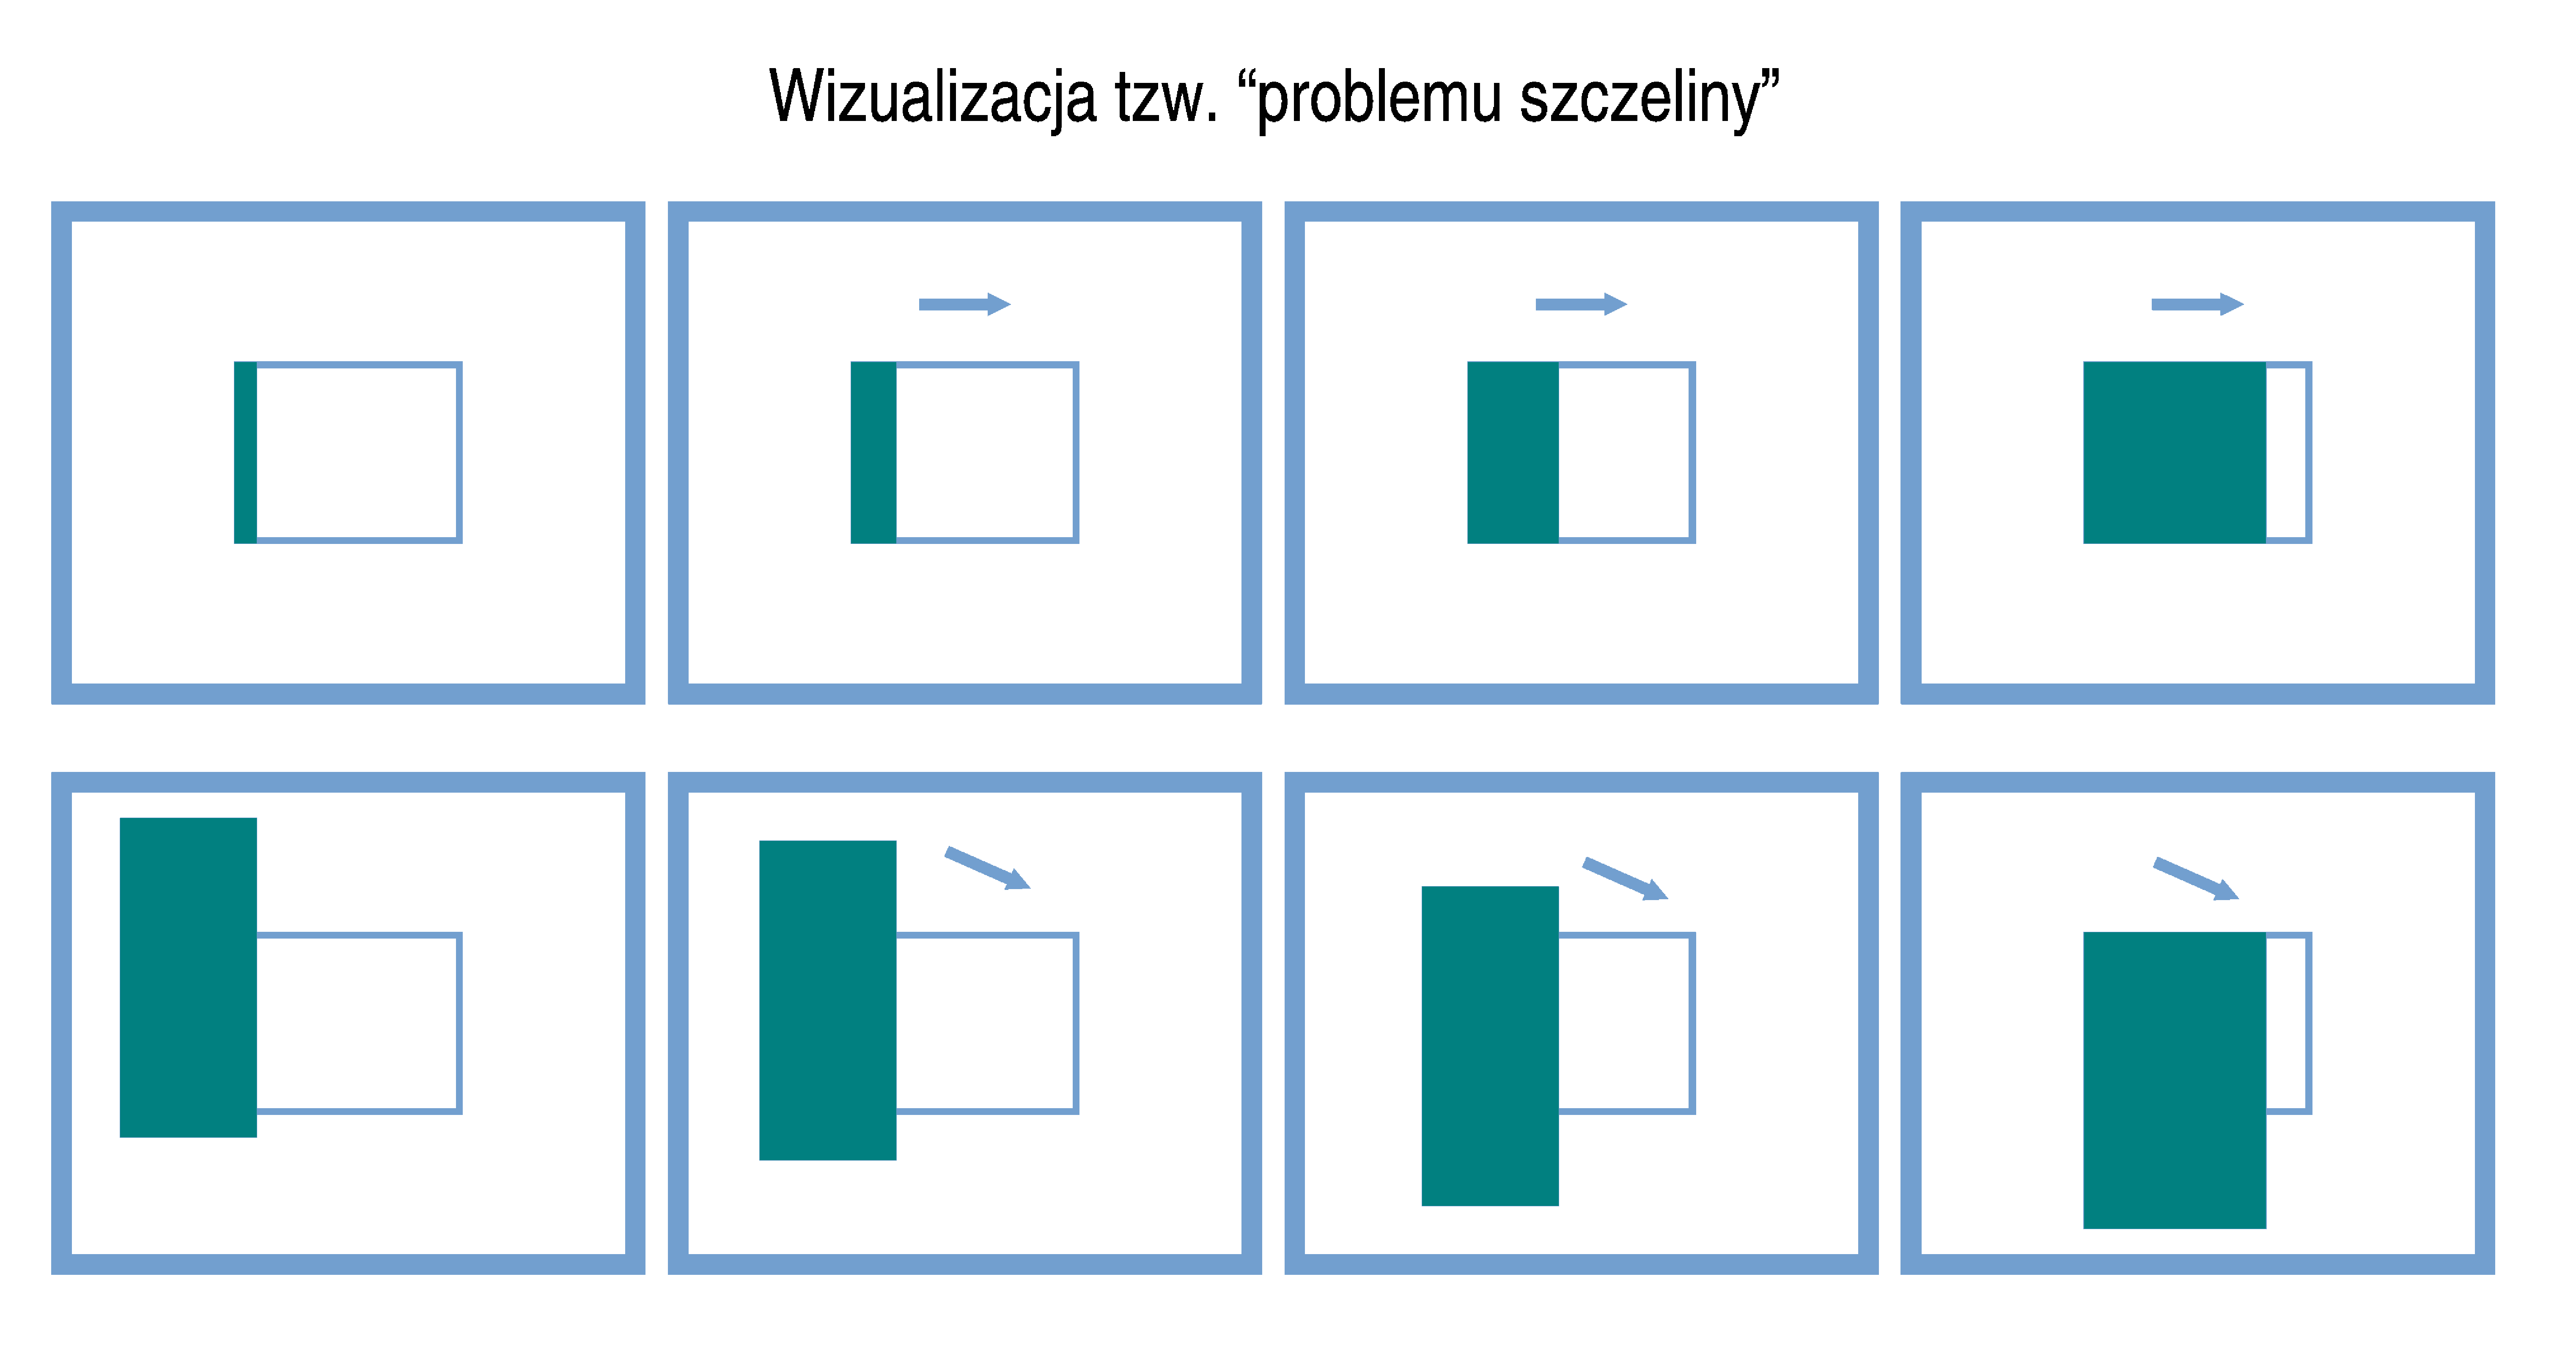
\includegraphics[width=14cm]{ApertureProblem}
      \caption[Wizualizacja tzw. problemu szczeliny]{Wizualizacja tzw. \textit{problemu szczeliny}}
      \label{fig:ApertureProblem}
    \end{figure}

  \newpage
  \section{Problem doboru cech dla algorytmów śledzenia punktów charakterystycznych}\label{Section_GoodGeaturesToTrack}
    Wybór punktów charakterystycznych dla problemu śledzenia ich w~sekwencji wideo jest kluczowym elementem z~punktu widzenia jakości wyznaczonego rozwiązania końcowego. Analizując sekwencję wideo jedynie ze strukturą o~powtarzalnej teksturze, wybór charakterystycznego elementu okaże się bardzo trudny. Wiele punktów będzie identycznych lub bardzo podobnych do siebie i~śledzenie jednego wybranego pomiędzy kolejnymi ramkami animacji jest z~góry skazane na porażkę. Z~drugiej strony, jeśli algorytm ma do dyspozycji unikalny fragment, wybierając go zwiększa szanse na odnalezienie go w~następnych ramkach.

    Podejście intuicyjne do tego problemu, polegające na poszukiwaniu odróżniającego się szczegółu jest krótkowzroczne. Przy wyborze charakterystycznej cechy metoda można kierować się dużą wartością pochodnej w~punkcie - tego typu wartości oznaczają najczęściej \textbf{krawędź}. Niestety, podstawowa cechą \textit{krawędzi} jest to, że wiele punktów leżących na niej posiada identyczne wartości (prowadzi to do tzw. problemu szczeliny, który omówiony został powyżej). Potrzebne są bardziej unikalne właściwości.

    Pierwsze podejście do problemu doboru cech pozwoliło na odkrycie bardzo ważną własności dotyczącą wartości pochodnej. Okazuje się, że jeśli wartości pochodnej w~dwóch równoległych do siebie kierunkach są duże, to dany punkt jest dużo bardziej unikalny w~skali całej ramki - nazywany jest wtedy \textbf{narożnikiem}.

    Najpowszechniej używana definicja \textit{narożnika} została przygotowana przez \textit{Harrisa} (szczegóły zawarte w~pracy \cite{Harris88}) i~z~niej również korzystają autorzy w~pracy \cite{GoodFeaturesToTrack94}.

    Definicja opiera się macierzy drugich pochodnych intensywności obrazu w~określonym punkcie ($\partial^2 x$, $\partial^2 y$, $\partial x\partial y$). W~szczególności możliwe jest obliczenie wartości wspominanych pochodnych dla całej ramki animacji tworząc w~ten sposób nową ramkę przechowującą wartości drugich pochodnych nazwaną \textit{obrazem Hesjanów}. Hesjan (lub dokładniej \textit{macierz Hessego}) zdefiniowana jest następująco ($I$ jest intensywnością piksela $p$ obrazu):

    \[
      H(p) =
        \begin{bmatrix}
          \frac{\partial^2 I}{\partial x^2} & \frac{\partial^2 I}{\partial x\partial y} \\
          \frac{\partial^2 I}{\partial x\partial y} & \frac{\partial^2 I}{\partial y^2} \\
        \end{bmatrix}_{p}.
    \]

    \newpage
    Dla powyższej definicji narożnika kolejnym ważnym elementem jest \textit{macierz autokorelacji drugich pochodnych} dla każdego śledzonego punktu otoczonego \textit{oknem} o~określonych, małych wymiarach. Macierz autokorelacji jest zdefiniowana w~następujący sposób ($w_{i,j}$ jest współczynnikiem zależnym od zastosowanego okna):

    \[
      M(x, y) =
        \begin{bmatrix}
            \displaystyle\sum\limits_{K \le i, j \le K}
              \scalemath{0.75}{w_{i,j} I_{x}^{2} (x + i, y + j)} &
            \displaystyle\sum\limits_{K \le i, j \le K}
              \scalemath{0.75}{w_{i,j} I_{x} (x + i, y + j) I_{y} (x + i, y + j)} \\

            \displaystyle\sum\limits_{-K \le i, j \le K}
              \scalemath{0.75}{w_{i,j} I_{x} (x + i, y + j) I_{y} (x + i, y + j)} &
            \displaystyle\sum\limits_{-K \le i, j \le K}
              \scalemath{0.75}{w_{i,j} I_{y}^{2} (x + i, y + j)} \\
        \end{bmatrix}.
    \]

    Przy tak zdefiniowanej \textit{macierzy autokorelacji} narożnikiem zgodnie z~definicją \textit{Harrisa} nazywane jest miejsce, dla którego powyższa macierz posiada \textit{dwie duże wartości własne}. Oznacza to, że w~danym punkcie istnieje krawędź (lub faktura) rozciągająca się w~dwóch kierunkach, tak jak w~przypadku rzeczywistego narożnika. Warto zauważyć, że dzięki zastosowaniu drugiej pochodnej całość jest niewrażliwa na stałą wartość pierwszej pochodnej (druga pochodna będzie wtedy równa $0$).

    Zastosowanie wartości własnych dla tej definicji ma kilka dodatkowych zalet. Dzięki wybraniu miejsc posiadających duże wartości własne (a~w konsekwencji wektory własne) wybrany fragment staje się niewrażliwy na rotację. Dodatkowo dwie duże wartości własne, stanowią same w~sobie bardzo dobre wartości do śledzenia w~przyszłych klatkach animacji.

    Badając definicję \textit{Harrisa} autorzy pracy \cite{GoodFeaturesToTrack94}, \textit{Shi} oraz \textit{Tomasi}, zauważyli, że dobrym \textit{narożnikiem} (w~sensie jakościowym) można nazwać taki element, którego mniejsza z~obliczonych wartości własnych jest zawsze większa od pewnego przyjętego \textit{minimalnego progu}. Taki sposób wyznaczania narożników daje w~większości przypadków dużo lepsze rezultaty niż oryginalna definicja. W~rozdziale \ref{Section_ImplementationDetails} została omówiona dokładnie procedura $goodFeaturesToTrack()$ korzystającą z~powyżej własności.

    Inną bardzo ważną definicją jest \textit{Skaloniezmiennicze przekształcenie cech} (ang. \textit{Scale-invariant feature transform}, w skrócie \textit{SIFT}) opisane w~pracy \cite{SalientPointsTracking05}. Ponadto, omawiany algorytm w~wariancie \textit{L\"{o}we}, odpornym na częściowe przesłanianie, jest opatentowanym algorytmem w~Stanch Zjednoczonych.

    Algorytm pozwala na wykrycie cech w~obrazie, które są odporne na skalowanie, rotację i~przesunięcie. W~przypadku ogólnym omawiane cechy obliczane są na podstawie kierunku dominującego gradientu w~określonym położeniu i~naniesieniu wartości do lokalnego histogramu na podstawie jego orientacji. Dzięki temu, przy odpowiednio małych przekształceniach afinicznych (w~omawianym przypadku, pomiędzy dwoma bezpośrednio sąsiadującymi klatkami sekwencji wideo) obserwowane cechy nie zmieniają się.

    Metoda została opracowana przez Davida L\"{o}we w~roku 1999. Ogólna idea algorytmu opiera się na wyekstrahowaniu punktów kluczowych do odpowiedniej struktury danych, następnie obiekt jest identyfikowany w~nowym obrazie pojedynczo, na podstawie odległości w~metryce euklidesowej oraz za pomocą wektora cech. Z~pełnego zbioru dopasowań wybierane zostają tylko te punkty, które zgadzają się pod względem położenia, skali i~orientacji. Dzięki zastosowaniu efektywnej struktury danych (w~proponowanej implementacji tablicy haszowanej) identyfikacja skupisk śledzonych punktów i~wybór tych najwierniej odpowiadających (za pomocą uogólnionej \textit{transformaty Hough}) oryginalnie śledzonemu obiektowi przebiega bezproblemowo. Następnie, każdy zidentyfikowany klaster trzech lub więcej punktów podlega weryfikacji hipotezy przynależności do śledzonego punktu. Skupiska nie pasujące do omawianej hipotezy zostają odrzucone, klastry wyznaczone przez poprzednie kroki z~poprawnie zweryfikowaną hipotezą z~dużym prawdopodobieństwem należą do śledzonego obiektu.

\chapter{Analiza i~porównanie wybranych algorytmów}\label{Section_Algorytmy}

  \section{Algorytmy oparte o~przepływ optyczny}\label{Subsection_OpticalFlow}

    \subsection{Ogólny zarys algorytmów opartych o~przepływ optyczny}
    Przy śledzeniu punktów charakterystycznych, bardzo często metody nie posiadają szczegółowej wiedzy o~środowisku i~obserwowanym podmiocie. W~takiej sytuacji własności algorytmów opartych o~przepływ optyczny sprawdzają się najlepiej, ponieważ sam ruch i~zmiany zachodzące pomiędzy kolejnymi klatkami animacji same w~sobie niosą najwięcej informacji\cite{OpticalFlowNonPriori05}. Poniżej zilustrowano zasadę działania przepływu optycznego.

    \begin{figure}[!ht]
      \centering
      \includegraphics[width=14cm]{OpticalFlowDescription}
      \caption[Ilustracja działania przepływu optycznego]{Ilustracja działania przepływu optycznego}
      \label{fig:OpticalFlowDescription}
    \end{figure}

    Przypisując wektor prędkości (lub przemieszczenie, różnicę odległości jaką piksel przebył od swojego ostatniego położenia w~poprzedniej ramce sekwencji wideo) do każdego piksela, tworzony jest obraz przepływu optycznego nazwany \textit{gęstym} (został on szczegółowo omówiony w~\ref{Subsection_DenseOpticalFlow}). Powstały obraz nazywany jest \textit{wektorowym polem prędkości}. Podczas obserwacji tego typu metod, łatwo zauważyć, że wiele wektorów prędkości na obrazie posiada długość $0$ (innymi słowy, piksele w~tych miejscach się nie poruszają) i~można pokusić się o~optymalizację metody gęstej poprzez wprowadzenie okna obserwacji nazwanego \textit{blokiem}. Taki rodzaj gęstego przepływu optycznego nosi nazwę \textit{dopasowywania bloków}, nie został on jednak wzięty pod uwagę w~przeprowadzonych badaniach.

    Obliczenie \textit{wektorowego pola prędkości} jest zadaniem złożonym obliczeniowo. Złożoność asymptotyczna wynosi $O(Cnm)$, gdzie $C$ jest stałą związaną z~obliczeniami wektora prędkości dla danego punktu, a~$n$ oraz $m$ są wymiarami klatki animacji. Omawiana stała posiada bardzo duży wpływ na końcową postać złożoności ze~względu na zastosowanie metody interpolacji między śledzonymi punktami w~celu uzyskania jednoznacznego rezultatu.

    Gęsty przepływ optyczny, mimo intuicyjnej definicji, jest metodą o~bardzo dużym koszcie obliczeniowym. Próba zredukowania obliczanego pola wektorów doprowadziła do stworzenia metody \textit{dopasowania bloków} omówionej powyżej. Intuicyjnie, możliwe jest jeszcze większe ograniczenie złożoności, poprzez śledzenie tylko charakterystycznej grupy punktów, oraz zastosowanie \textit{definicji narożnika} omówionej szczegółowo w~rozdziale \ref{Section_GoodGeaturesToTrack} oraz artykułach \cite{LucasKanadeTracker81} i~\cite{GoodFeaturesToTrack94}. Właśnie takie sformułowanie problemu nazywane jest \textit{rzadkim przepływem optycznym}. Koszt obliczeniowy jest dużo mniejszy niż w~przypadku gęstego przepływu i~jest wprost proporcjonalny do mocy zbioru punktów charakterystycznych, która w~zdecydowanej większości przypadków jest dużo mniejsza od ilości punktów obrazu.

    Poniżej zostały szczegółowo omówione algorytmy przepływu optycznego rzadkiego oraz gęstego.

    \subsection{Rzadki przepływ optyczny (algorytm Lucas-Kanade)}
    Oryginalna idea algorytmu opracowanego przez parę \textit{Lucas} - \textit{Kanade} (\textit{LK}) została zaproponowana w~1981 roku w~pracy \cite{LucasKanadeTracker81} i~początkowo była próbą stworzenia algorytmu wariantu \textit{gęstego} o~mniejszej złożoności obliczeniowej. Poprzez łatwość zaaplikowania reguł stworzonej metody do listy punktów charakterystycznych obrazu wejściowego została jedną z~najważniejszych metod wariantu \textit{rzadkiego}.

    Algorytm \textit{LK} może zostać wykorzystany jako przepływ optyczny typu \textit{rzadkiego}, ponieważ wszystkie jego własności opierają się tylko i~wyłącznie na lokalnym kontekście, w~tzw. \textit{oknie} otaczającym śledzony punkt. Właśnie ta własność może być również najpoważniejszą wadą algorytmu, gdy zostanie zastosowane okno o~zbyt małych rozmiarach (punkt w~kolejnej klatce animacji może znaleźć się poza rozważanym oknem, dochodzi również problem \textit{szczeliny} i~niejednoznaczności przy analizie kierunku ruchu w~takiej sytuacji).

    Aby uniknąć sytuacji, w~której dobrane okno jest zbyt małe stosuje się tzw. wariant \textit{piramidalny} algorytmu \textit{LK} opisany dokładnie w~pracy \cite{OpenCvOpticalFlow04}. Na wstępie dla aktualnej klatki animacji budowana jest piramida obrazów o~stopniowanej jakości oraz rozmiarze. Śledzenie rozpoczyna się od największego i~najmniej szczegółowego obrazu stopniowo przechodząc do mniejszych, bogatszych w~szczegóły stopni piramidy. Dzięki temu, szybszy i~bardziej dynamiczny ruch może zostać złapany nawet poprzez mniejsze okna dookoła punktów charakterystycznych.

    \newpage
    Algorytm rzadkiego przepływu optycznego zaproponowany przez parę \textit{Lucas} - \textit{Kanade} został oparty na trzech podstawowych definicjach:
    \begin{itemize}
      \item Twierdzenie o~stałej jasności - śledzony piksel obrazu nie zmienia swojej jasności (w~przypadku analizy obrazów kolorowych reguła nosi nazwę \textit{Reguły niezmienności koloru}) podczas ruchu pomiędzy klatkami.
      \item Twierdzenie o~niewielkim ruchu - śledzony fragment powierzchni porusza się o~niewielką odległość z~klatki na klatkę. Innymi słowy, \textit{ilość klatek sekwencji wideo} jest na tyle wysoka, aby transformacja śledzonego punktu pomiędzy dwoma ramkami była wykonywana na małym fragmencie całego obrazu klatki.
      \item Twierdzenie o~jednolitej przestrzeni - punkty sąsiadujące z~śledzonym należą do tej samej powierzchni, poruszającej się zgodnie z~tym samym wektorem prędkości i~są rzutowane w~bezpośredniej bliskości punktu charakterystycznego.
    \end{itemize}

    Dla uproszczenia wyjaśnień przyjęty został obraz w~skali szarości o~jednym kanale opisanym liczbą zmiennoprzecinkową.

    Pierwsze twierdzenie wymaga aby śledzony punkt danej powierzchni wyglądał tak samo w~kolejnych klatkach animacji (inaczej: wyglądał tak samo w~czasie), co matematycznie zapisane jest następująco: \[ f(x, t) \equiv I(x(t), t) = I(x(t + dt), t + dt), \] co oznacza, że jasność śledzonego punktu nie ulega zmianom w~czasie: \[ \frac{\partial f(x)}{\partial t} = 0. \]

    Drugi warunek oznacza, że ruch wybranego punktu z~ramki na ramkę jest \textit{mały}. Innymi słowy, zmiana jest aproksymacją pochodnej intensywności obrazu w~dziedzinie czasu (założone zostało, że omawiana zmiana jest \textit{różniczkowalna}). Aby wyjaśnić konsekwencje tego założenia, najpierw zostanie opisany przypadek jednowymiarowy.

    W~przestrzeni jednowymiarowej została wykorzystana pierwsza definicja, zastępując funkcję jasności $f(x,t)$ wyrażeniem $I(x(t), t)$ oraz zakładając zależność zmiennej $x$ od $t$. Po skorzystaniu z~twierdzenia o~pochodnej funkcji złożonej otrzymano: \[ \underbrace{ \left. \frac{\partial I}{\partial x}\right|_{t} }_{I_{x}} \underbrace{ \left(\frac{\partial x}{\partial t}\right) }_{\mathbf{v}} + \underbrace{ \left. \frac{\partial I}{\partial t}\right|_{x(t)} }_{I_{t}} = 0, \] gdzie $I_{x}$ jest pochodną pierwszego obrazu, $I_{t}$ jest pochodną obrazu następnej klatki, a~$\mathbf{v}$ jest poszukiwanym wektorem prędkości. Po przekształceniu uzyskano równanie dla przypadku jednowymiarowego: \[ \mathbf{v} = -\frac{I_{t}}{I_{x}}. \]

    \newpage
    Obserwując krawędź w~przypadku jednowymiarowym, jak na rysunku \ref{fig:EdgeVelocity1D}, poruszając się wzdłuż osi $x$ od większych wartości po lewej stronie w~stronę wartości mniejszych po stronie prawej. Jak zdefiniowano powyżej, poszukiwana jest prędkość $\mathbf{v}$ z~jaką punkt na krawędzi się porusza. Zgodnie z~obliczeniami w~miarę poruszania się wzdłuż osi odciętych szybkość rośnie wraz z~nachyleniem. Dodatkowo ujemny znak kompensuje nachylenie.

    \begin{figure}[!ht]
      \centering
      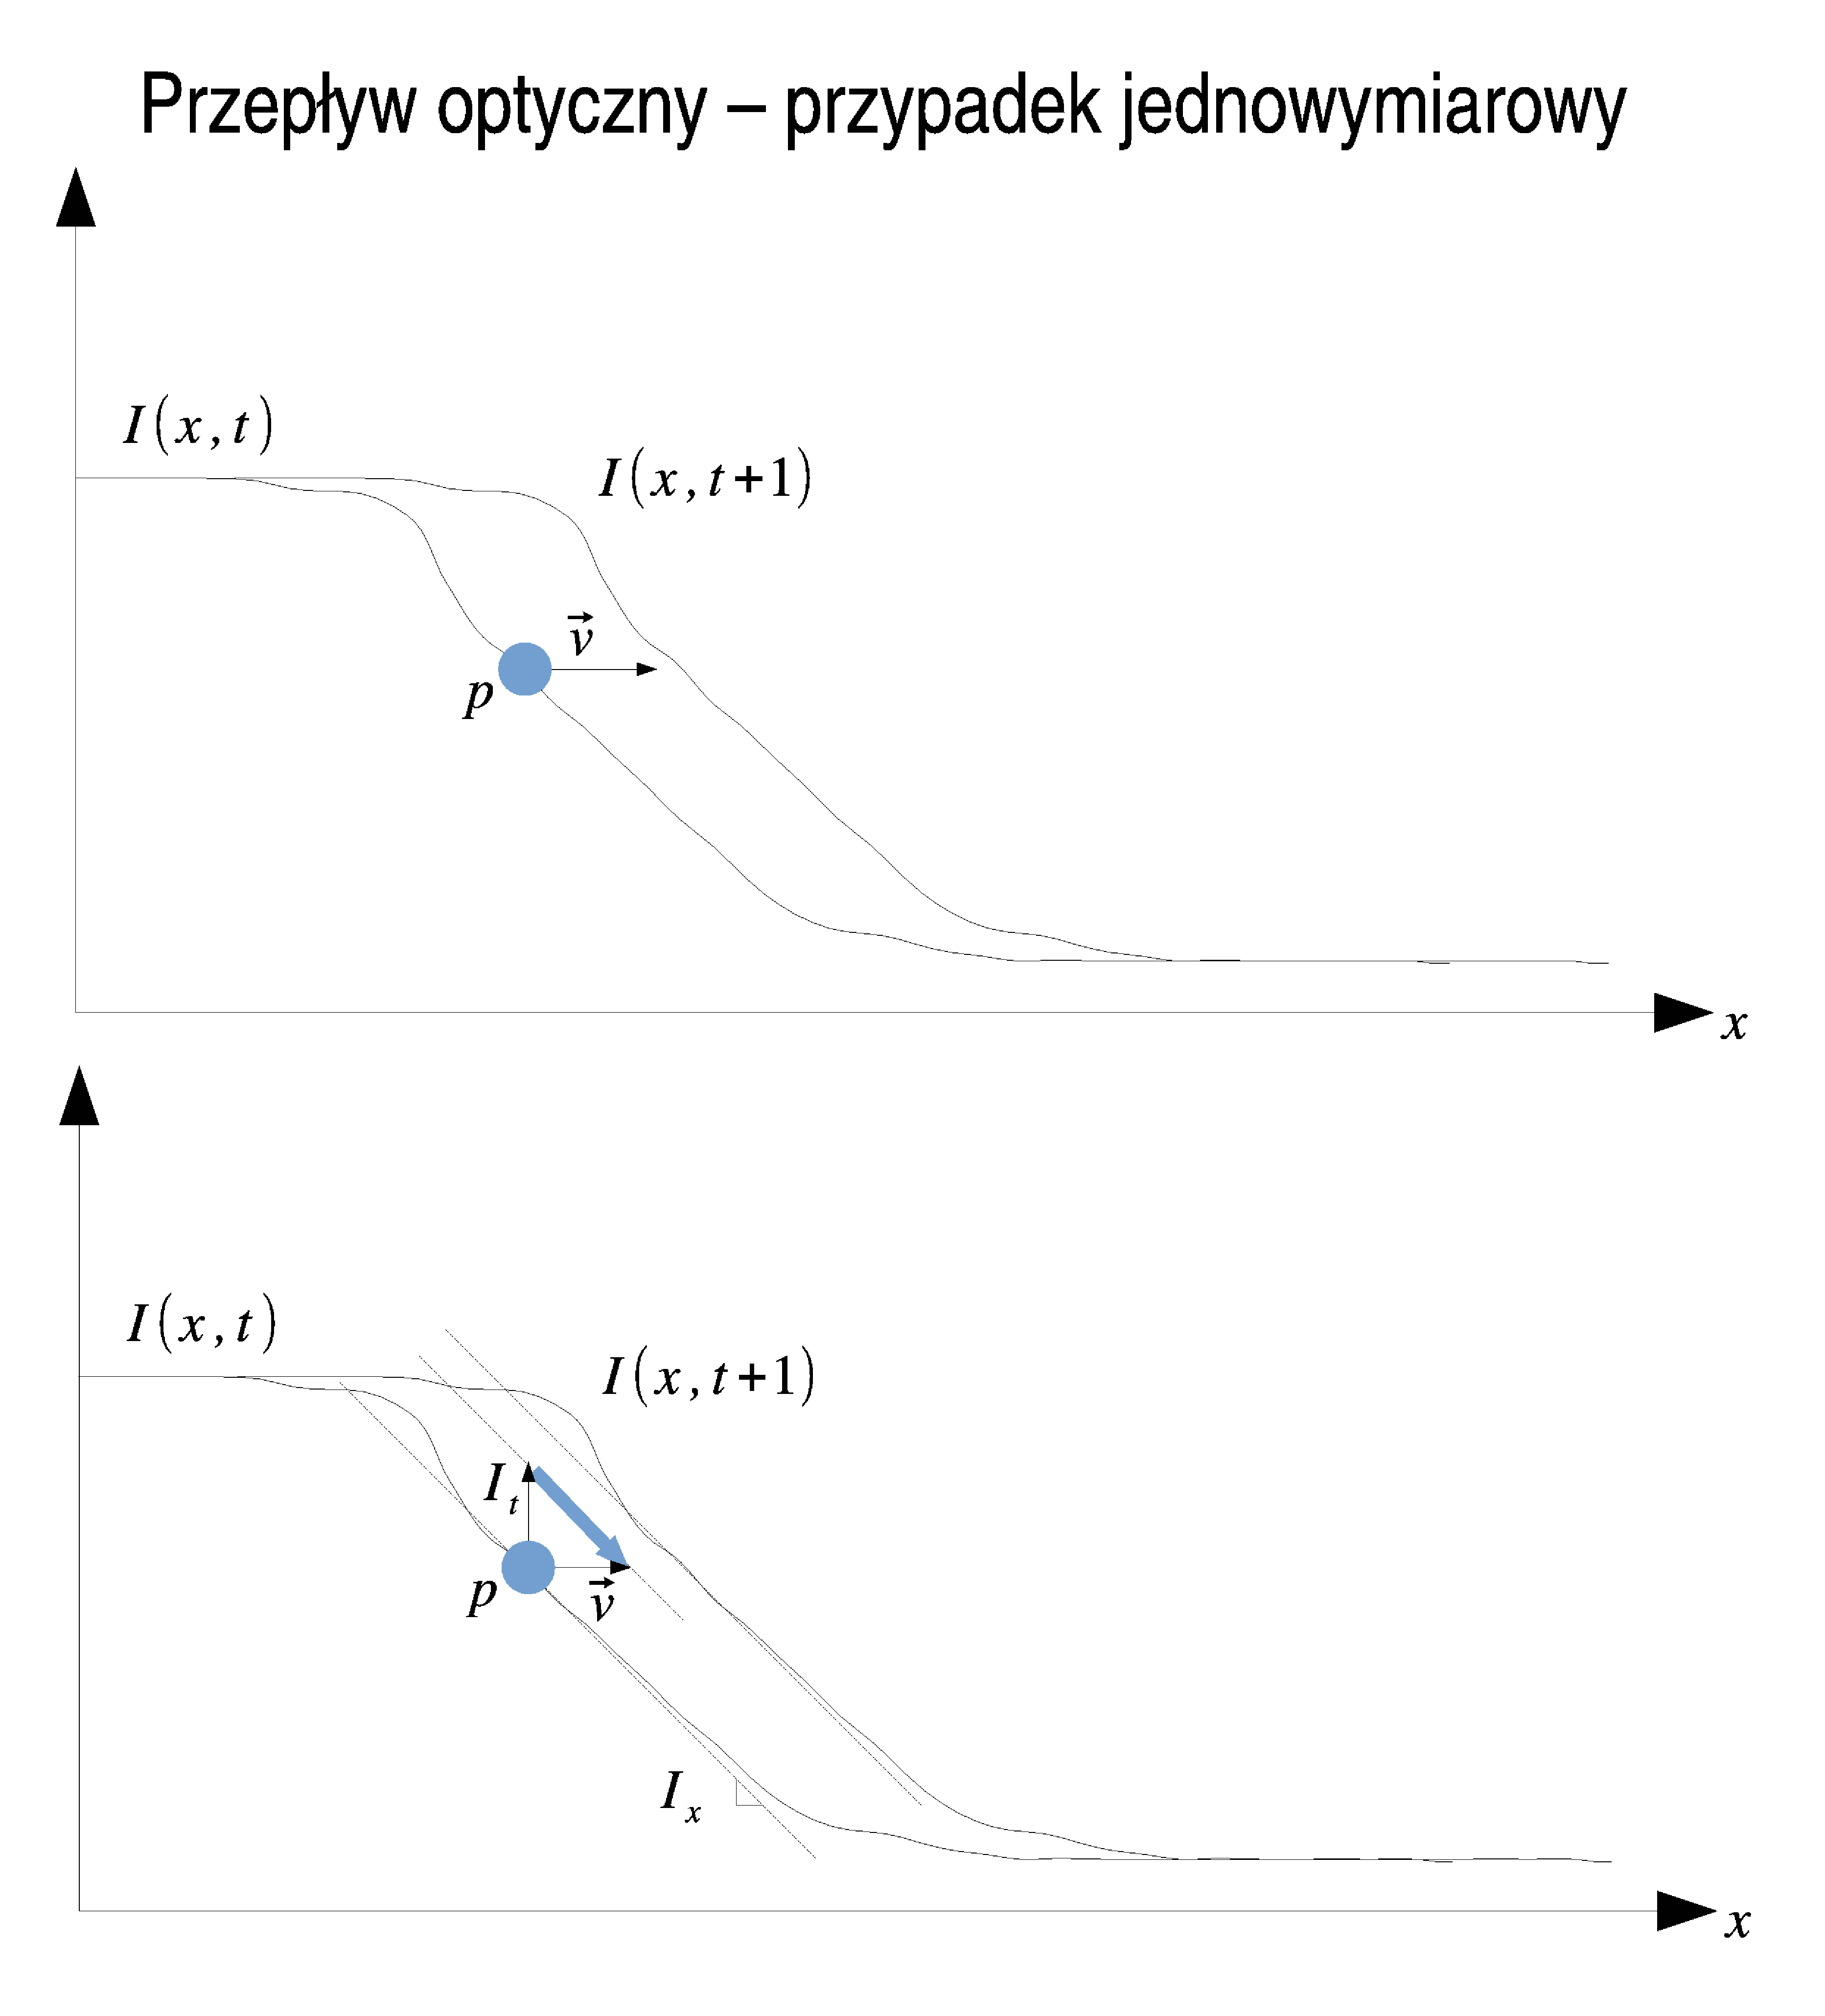
\includegraphics[width=14cm]{EdgeVelocity1D}
      \caption[Wizualizacja pomiaru szybkości poruszania się krawędzi dla przypadku jednowymiarowego]{Wizualizacja pomiaru szybkości poruszania się krawędzi dla przypadku jednowymiarowego}
      \label{fig:EdgeVelocity1D}
    \end{figure}

    Niestety, jasność nie zawsze będzie stała, i~poczynione założenie nie będzie w~takim przypadku prawdziwe - w~konsekwencji nie otrzymano dokładnego wektora prędkości. Natomiast dla małych odległości możliwe jest przybliżenie rozwiązania za pomocą \textit{iteracyjnej metody Newtona}, obliczając kolejne pochodne po czasie. Przy założeniu, że kolejne klatki reprezentują niewielki ruch, rozwiązanie jest szybko zbieżne (wystarcza około 5 iteracji), jeśli jednak pierwsze przybliżenie będzie niedokładne, zaproponowana metoda będzie rozbieżna.

    \begin{figure}[!ht]
      \centering
      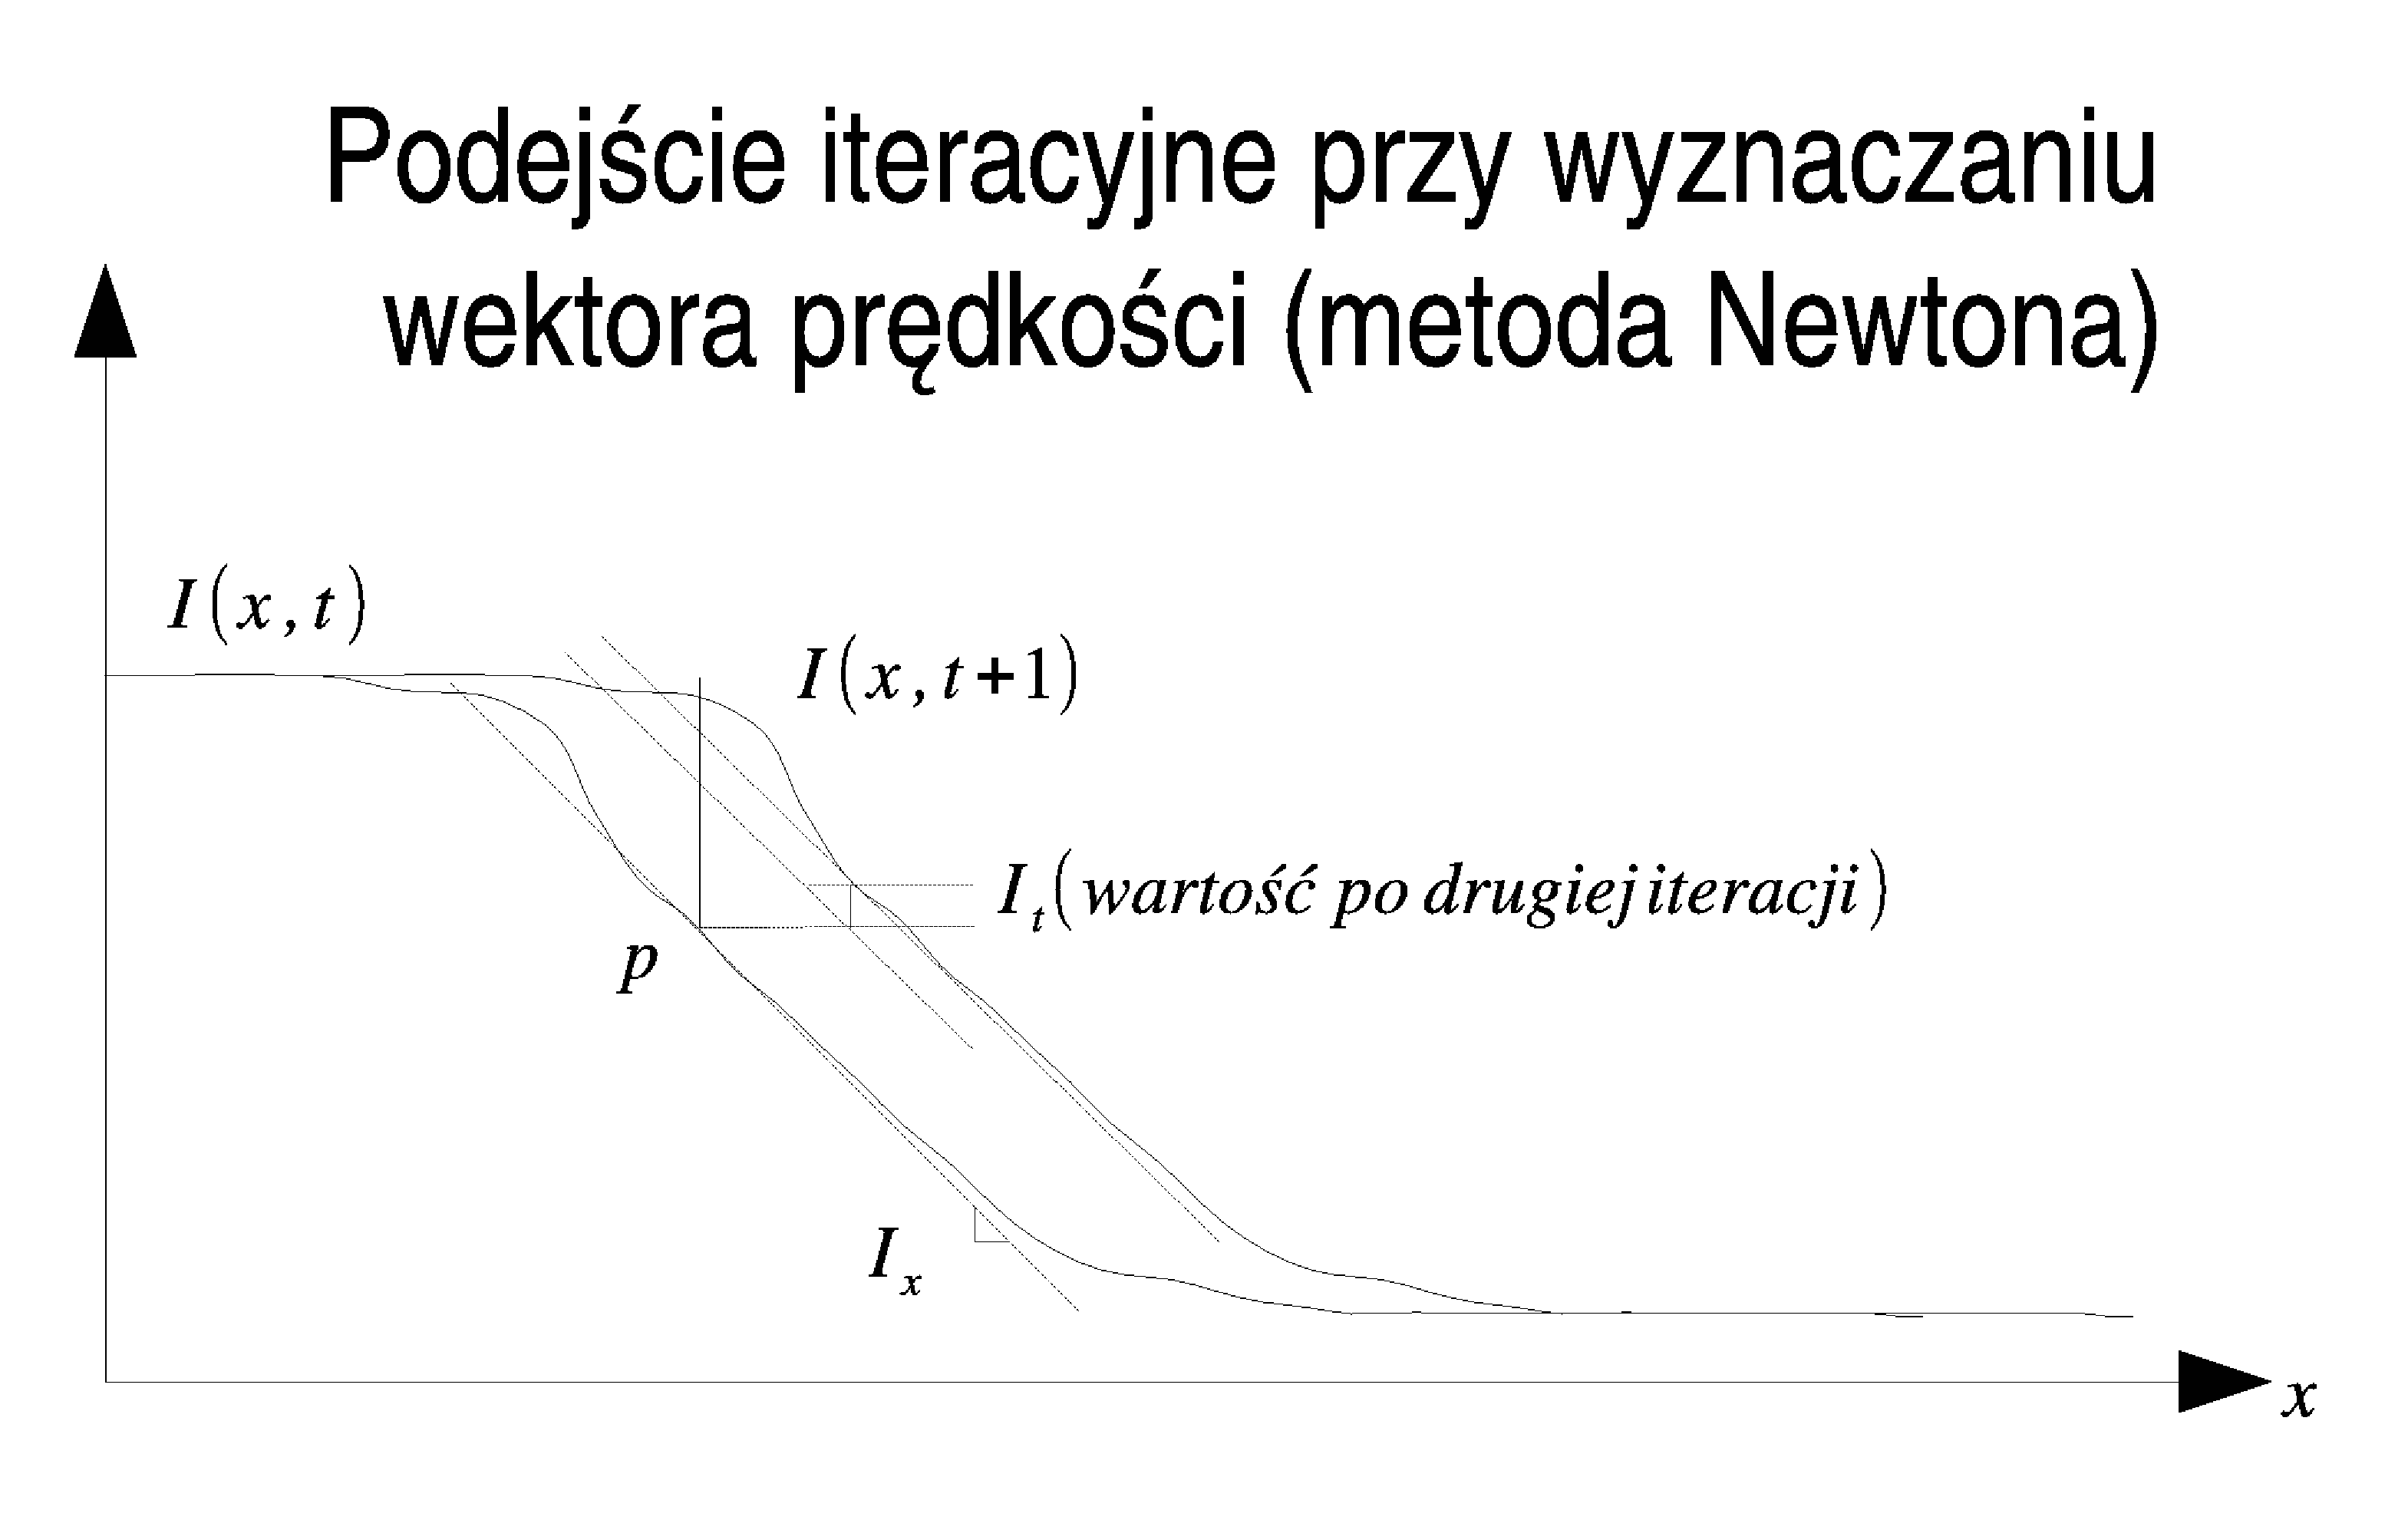
\includegraphics[width=14cm]{Iterations}
      \caption[Podejście iteracyjne przy wyznaczaniu wektora prędkości]{Podejście iteracyjne przy wyznaczaniu wektora prędkości}
      \label{fig:Iterations}
    \end{figure}

    Próba przeniesienia proponowanego rozwiązania na przypadek dwuwymiarowy wymaga dodania współrzędnej $y$, co modyfikuje opisane równanie do postaci: \[I_{x}\mathbf{u} + I_{y}\mathbf{v} + I_{t} = \mathbf{0}. \]

    Niestety równanie w~tej postaci jest niedookreślone, ponieważ dla każdego piksela są obecne dwie niewiadome. Oznacza to, że na poziomie pojedynczych pikseli nie jest możliwe uzyskanie dokładnego rozwiązania dla ruchu w~przestrzeni dwuwymiarowej. W~takim przypadku możliwe jest jedynie rozwiązanie składnika ruchu który jest równoległy do linii, wyznaczonej przez równanie przepływu, co jest zaprezentowane poniżej:

    \[ I_{x}\mathbf{u} + I_{y}\mathbf{v} + I_{t} = \mathbf{0}, \]

    \[ \nabla \mathbf{I}^{T} \mathbf{u} = -\mathbf{I_{t}}, \]
    \[
      \mathbf{u} =
        \begin{bmatrix}
          u \\
          v \\
        \end{bmatrix}
      \hspace{20pt}
      \nabla \mathbf{I} =
        \begin{bmatrix}
          I_{x} \\
          I_{y} \\
        \end{bmatrix}.
    \]

    Aby rozwiązać przypadek dwuwymiarowy bez wspomnianego problemu, niezbędne jest skorzystanie z~trzeciego twierdzenia o~jednolitej przestrzeni. Jeśli grupa pikseli porusza się z~identyczną prędkością i~należy fizycznie do jednego obiektu, możliwe jest wykorzystanie ich własności do rozwiązania omawianego równania, poprzez zastosowanie okna (najczęstszy wybór to: 3 na 3, 5 na 5 lub 7 na 7 pikseli), dla którego w~centrum znajduje się śledzony punkt. Dla okna o~rozmiarze 3 na 3 uzyskano 9 dodatkowych równań, dzięki czemu niedookreślony układ równań staje się nadokreślony, co zostało zilustrowane poniżej:

    \[
      \underbrace{
        \begin{bmatrix}
          I_{x}(p_{1}) & I_{y}(p_{1}) \\
          I_{x}(p_{2}) & I_{y}(p_{2}) \\
          \vdots       & \vdots       \\
          I_{x}(p_{9}) & I_{y}(p_{9}) \\
        \end{bmatrix}}_{\substack{A\\9x2}}
      \underbrace{
        \begin{bmatrix}
          \mathbf{u} \\
          \mathbf{v} \\
        \end{bmatrix}}_{\substack{\mathbf{d}\\2x1}} =
      -\underbrace{
        \begin{bmatrix}
          I_{t}(p_{1}) \\
          I_{t}(p_{2}) \\
          \vdots       \\
          I_{t}(p_{9}) \\
        \end{bmatrix}}_{\substack{\mathbf{b}\\9x1}}.
    \]

    Aby rozwiązać zadany układ równań zastosowano metodę najmniejszych kwadratów zgodnie z~$min||Ad - b||^{2}$ co daje:

    \[
      \underbrace{(A^{T}A)}_{2x2} \underbrace{d}_{2x1} = \underbrace{A^{T}b}_{2x2}.
    \]

    Następnie wyłączone zostały poszukiwane wektory $\mathbf{v}$ oraz $\mathbf{u}$:

    \[
      \underbrace{
        \begin{bmatrix}
          \sum I_{x} I_{x} & \sum I_{x} I_{y} \\
          \sum I_{x} I_{y} & \sum I_{y} I_{y} \\
        \end{bmatrix}
      }_{A^{T}A}
      \begin{bmatrix}
        \mathbf{u} \\
        \mathbf{v} \\
      \end{bmatrix} =
      -\underbrace{
        \begin{bmatrix}
          \sum I_{x} I_{t} \\
          \sum I_{y} I_{t} \\
        \end{bmatrix}
      }_{A^{T}b}.
    \]

    Co ostatecznie prowadzi do rozwiązania:

    \[
      \begin{bmatrix}
        \mathbf{u} \\
        \mathbf{v} \\
      \end{bmatrix} = (A^{T}A)^{-1} A^{T}b.
    \]

    Aby rozwiązać powyższe równanie część $(A^{T}A)$ musi być odwracalna, a~warunek odwracalności zostanie spełniony wtedy i~tylko wtedy gdy omawiany fragment posiada rząd równy $2$. Powyższe wymaganie zostanie spełnione, gdy wspomniana macierz posiada dwa duże wektory własne. Przywołując \textit{definicję Harrisa} z~rozdziału \ref{Section_GoodGeaturesToTrack} dokładnie takie własności uzyskano tworząc okno wokół śledzonego punktu, który jest \textit{narożnikiem}. Z~wykorzystaniem takiego piksela jest możliwe rozwiązanie powyższego układu równań, wyznaczając wektory prędkości w~dwuwymiarowej przestrzeni.

    Ostatnim problemem jest zachowanie trzech twierdzeń dla obrazów gorszej jakości. Większości kamer dostępnych dla użytkowników końcowych pracuje z~częstotliwością 30 Hz, więc duże i~niespójne obszary ruchu są powszechnym problemem. Czysta implementacja algorytmu rzadkiego przepływu optycznego Lucas-Kanade nie radzi sobie z~takim rodzajem zakłóceń zbyt dobrze (problemem jest rozmiar okna, które zwiększone do dużych rozmiarów, aby objęło cały duży i~niespójny obszar ruchu łamie trzecie twierdzenie). Rozwiązaniem problemu jest wykorzystanie wariantu algorytmu \textit{LK} zwanego \textit{piramidalnym}, ze względu na zastosowaną konstrukcję wewnątrz implementacji algorytmu. Na rysunku \ref{fig:OpticalFlowPyramids} zaprezentowana została wizualizacja omawianej struktury.

    \begin{figure}[!ht]
      \centering
      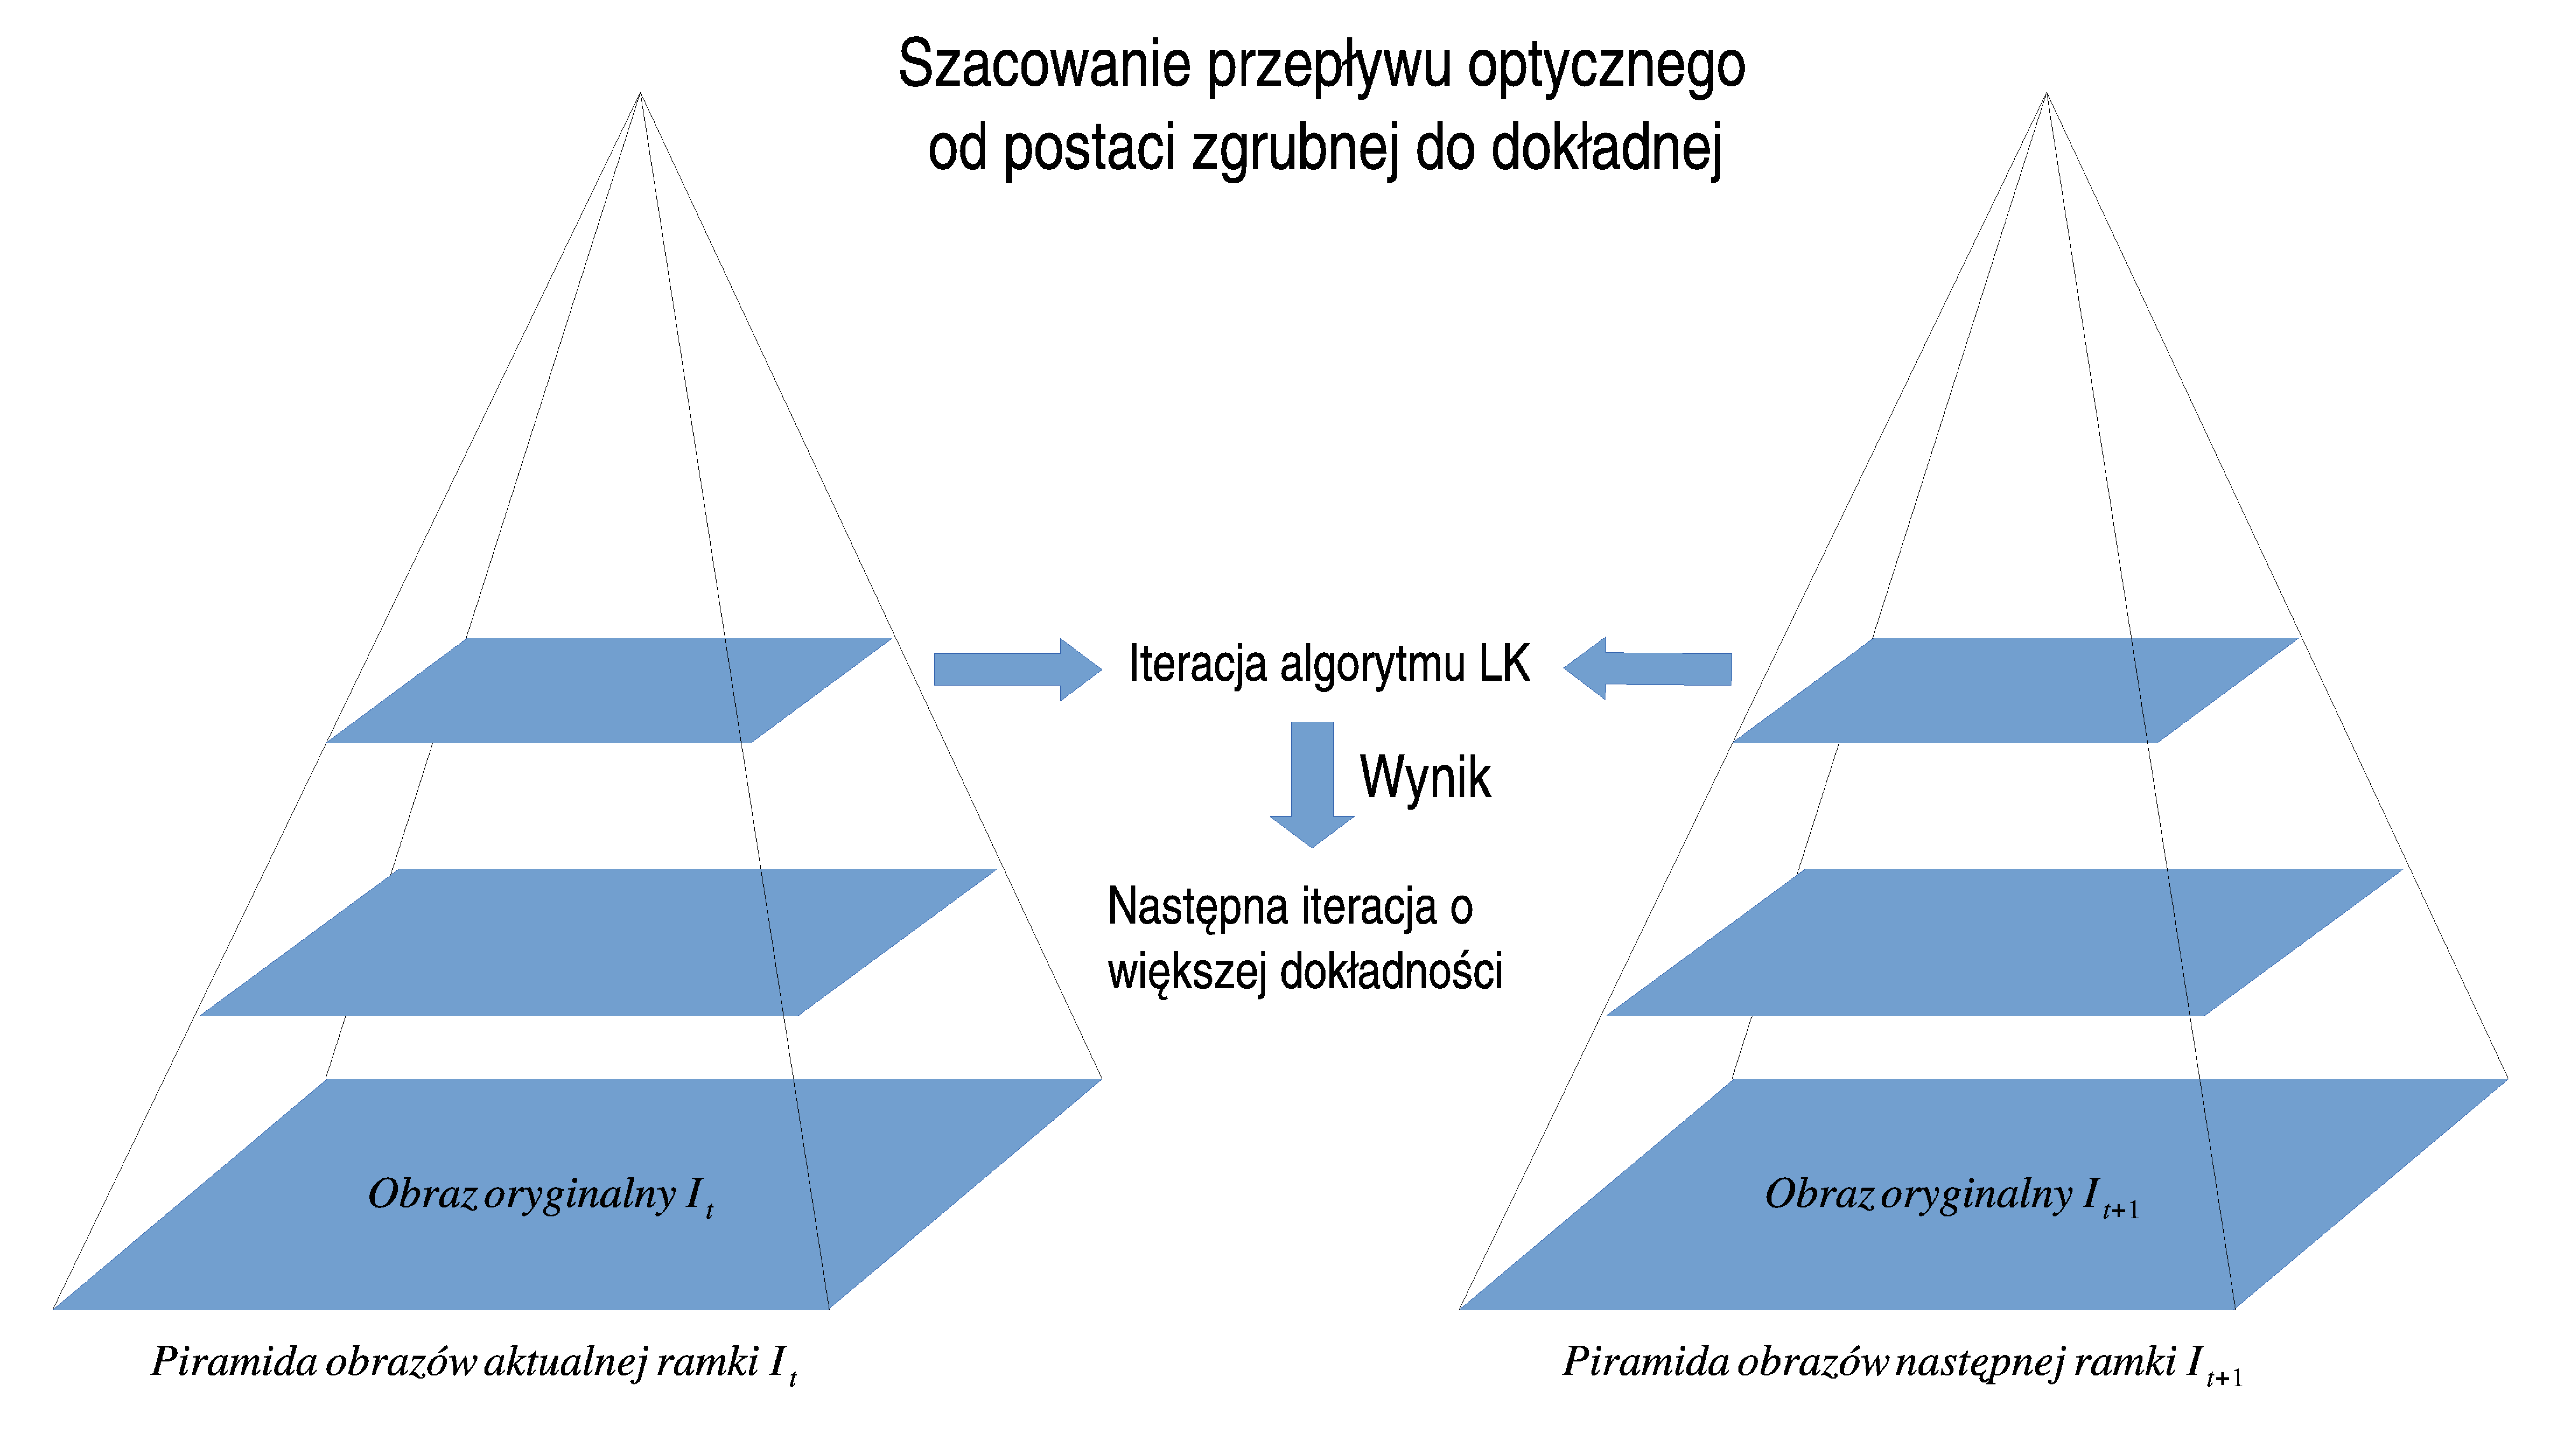
\includegraphics[width=14cm]{OpticalFlowPyramids}
      \caption[Prezentacja koncepcji piramid wykorzystywanych w~algorytmie \textit{Lucas}-\textit{Kanade}]{Prezentacja koncepcji piramid wykorzystywanych w~algorytmie \textit{Lucas}-\textit{Kanade}. Estymacja przepływu optycznego od reprezentacji zgrubnej do szczegółowej}
      \label{fig:OpticalFlowPyramids}
    \end{figure}

    Algorytm w~wariancie \textit{piramidalnym} tworzy dwie struktury dla aktualnej i~następnej ramki. Następnie przegląda dostępne klatki animacji od najmniejszej (najwyższej) do największej, najbardziej szczegółowej (najniższej). Dzięki temu eliminuje problemy związane z~naruszeniem drugiego twierdzenia (o~małym ruchu pomiędzy klatkami). Oszacowane wartości pojawiające się po analizie mniej szczegółowej ramki są wejściem do analizy ramki umieszczonej na następnym poziomie, dzięki temu za pomocą kolejnych poziomów obliczone rozwiązanie jest coraz bardziej dokładne.

    \subsection{Gęsty przepływ optyczny (algorytm Farnebäcka)}\label{Subsection_DenseOpticalFlow}
    Idea algorytmu gęstego przepływu optycznego wydaje się dużo bliższa intuicji, jednak przez próbę obliczenia pola wektorów prędkości dla całej klatki obrazu jest metodą dużo bardziej kosztowną obliczeniowo. W~przypadku omówionego wyżej algorytmu w~wersji \textit{rzadkiej} stworzonych zostało wiele założeń, które nie zostaną nigdy spełnione w~niektórych realnych zastosowaniach. Algorytm Farnebäcka opisany szczegółowo w~pracy \cite{GunnarFarneback03} powstał właśnie z~takiej potrzeby. Motywacją do stworzenia algorytmu była praca w~warunkach gdzie kamera wystawiona była na duże drgania i~obraz posiadał dużo zakłóceń z~tego powodu.

    Pierwszym krokiem algorytmu jest aproksymacja sąsiedztwa w~obu klatkach sekwencji wideo za pomocą wielomianów czwartego stopnia, do czego zastosowano rozwinięcie wielomianowe. Dzięki obserwacji jak nowo wyliczony wielomian zachowuje się po wprowadzeniu przesunięcia i~wprowadzeniu omówionych poniżej poprawek uzyskano wydajny i~dokładny algorytm gęstego przepływu optycznego.

    Podstawowa idea algorytmu opiera się na przybliżeniu sąsiedztwa każdego piksela za pomocą wielomianu. Jednocześnie wykorzystane zostają własności wielomianów czwartego stopnia, dzięki którym otrzymano lokalne wartości, w~lokalnym układzie współrzędnych. Formalizując powyższy opis, otrzymano \[ f(\mathbf{x}) \approx \mathbf{x}^{T}\mathbf{A}\mathbf{x} + \mathbf{b}^{T}\mathbf{x} + c, \] gdzie $\mathbf{A}$ jest macierzą symetryczną, $\mathbf{b}$ wektorem a $c$ skalarem. Odpowiednie współczynniki są oszacowane na podstawie ważonej metody najmniejszych kwadratów, pod względem dopasowania do wartości sygnału w~sąsiedztwie badanego piksela.

    Po przybliżeniu za pomocą wielomianu otoczenia badanego punktu, należy zbadać jak stworzona struktura zachowa się pod wpływem idealnego przesunięcia. Mając dany wielomian: \[ f_{1}(\mathbf{x}) = \mathbf{x}^{T}\mathbf{A_{1}}\mathbf{x} + \mathbf{b_{1}}^{T}\mathbf{x} + c_{1} \] stworzony został nowy, poddając pierwszy przesunięciu o~wartość $\mathbf{d}$: \[
      f_{2}(\mathbf{x}) = f_{1}(\mathbf{x-d}) = (\mathbf{x-d})^{T}\mathbf{A_{1}}(\mathbf{x-d}) + \mathbf{b_{1}}^{T}(\mathbf{x-d}) + c_{1}
    \] następnie, po przekształceniu otrzymano: \[
        f_{2}(\mathbf{x}) = \mathbf{x}^{T}\mathbf{A_{1}}\mathbf{x} + (\mathbf{b}_{1} - 2\mathbf{A}_{1}d)^{T}\mathbf{x} + \mathbf{d}^{T}\mathbf{A}_{1}\mathbf{d} - \mathbf{b}_{1}^{T}\mathbf{d} + c_{1}
    \] i~na koniec, po wykonaniu podstawienia, doprowadzono wielomian do postaci: \[
        f_{2}(\mathbf{x}) = \mathbf{x}^{T}\mathbf{A_{2}}\mathbf{x} + \mathbf{b_{2}}^{T}\mathbf{x} + c_{2},
    \] gdzie podstawione wartości wynoszą odpowiednio:
    \[ \mathbf{A}_{2} = \mathbf{A}_{1}, \]
    \[ \mathbf{b}_{2} = \mathbf{b}_{1} - 2\mathbf{A}_{1}\mathbf{d}, \]
    \[ c_{2} = \mathbf{d}^{T}\mathbf{A}_{1}\mathbf{d} - \mathbf{b}_{1}^{T}\mathbf{d} + c_{1}. \]

    Dzięki zaprezentowanej definicji $\mathbf{b}_{2}$ można obliczyć przesunięcie $\mathbf{d}$, jeśli macierz $\mathbf{A}_{1}$ jest odwracalna, zgodnie z~przekształceniami:
    \begin{equation}\label{Equation_GeneralDenseOpticalFlow}
      2\mathbf{A}_{1}\mathbf{d} = -(\mathbf{b}_{2} - \mathbf{b}_{1})
    \end{equation},
    \[ \mathbf{d} = -\frac{1}{2}\mathbf{A}_{1}^{-1}(\mathbf{b}_{2} - \mathbf{b}_{1}) \].
    Co najważniejsze, obserwacja jest możliwa do zaaplikowania w~każdym wymiarze (przypadek uogólniony).

    Mimo, iż zaprezentowany przypadek jest czysto teoretyczny (przez wprowadzone założenia, że \textit{sygnał jest pojedynczym wielomianem} oraz, że \textit{dwa sygnały łączy jedynie przesunięcie}) to jest nadal możliwy do zaaplikowania dla sygnału rzeczywistego. Jedynym wyzwaniem jest, aby dla równania \ref{Equation_GeneralDenseOpticalFlow} jak najbardziej ograniczyć wpływ błędów na wartość obliczonego przesunięcia. Aby ograniczyć wpływ błędu na wartość końcową wykorzystuje się ważoną metodę najmniejszych kwadratów dla sąsiedztwa analizowanego piksela. Dodatkowym ulepszeniem jest możliwość parametryzacji przesunięcia pod kątem doboru parametru dla określonych typów ruchu.

    Ostatnie założenie dotyczące \textit{ograniczenia natury różnicy pomiędzy dwoma sygnałami} może zostać wyeliminowane poprzez zastosowanie wiedzy \textit{a~priori} na temat ruchu. Nie ma ograniczeń co do porównania wielomianów obliczonych w~tym samym punkcie, więc korzystając z~wartości przemieszczenia zaokrąglonego do części całkowitej możemy obliczyć pierwsze oszacowanie a~następnie skupić się tylko na różnicy pomiędzy estymacją a~wartością docelową (różnica będzie dużo mniejsza).

    W~celu zoptymalizowania algorytmu, Farnebäck zaproponował podobne rozwiązanie jak w~\textit{piramidalnym wariancie algorytmu Lucas-Kanade} polegające na wykorzystaniu iteracyjnego podejścia i~piramidy przeskalowanych obrazów. Tak jak w~powyższym przypadku, algorytm zaczyna od mniej szczegółowych ramek, przechodząc co iterację do coraz bardziej szczegółowych obrazów.

  \section{Algorytm oparty o~lasy drzew losowych}\label{Subsection_RandomizedTrees}

    \subsection{Ogólny zarys algorytmów opartych o~drzewa decyzyjne}
    Kolejnym rozwiązaniem zaimplementowanym w~pracy jest algorytm śledzenia punktów charakterystycznych oparty o~lasy drzew losowych. W~porównaniu do problemu przepływu optycznego jest to zupełnie inna rodzina algorytmów, oparta o~uczenie maszynowe. Nie analizuje ona parami kolejnych ramek w~sekwencji wideo, a~klasyfikuje punkty charakterystyczne w~aktualnie przetwarzanej klatce animacji na podstawie określonej struktury reprezentującej wiedzę, która została zbudowana wcześniej, na podstawie określonego zbioru treningowego i~jej skuteczność została zweryfikowana za pomocą zbioru testowego.

    Celem uczenia maszynowego jest przekształcenie zbioru danych w~informacje, poprzez wyodrębnienie z~niego wzorców lub reguł. Po zbudowaniu struktury reprezentującej wiedzę za~pomocą wejściowego zbioru danych, maszyna z~jej pomocą powinna odpowiedzieć na określone pytanie na temat danych. Przykładowo, może to być pytanie o~stopień podobieństwa innego zestawu danych do danych, na podstawie których zbudowano bazę wiedzy.

    Bardzo rzadko algorytmy uczenia maszynowego działają na surowych, nieprzetworzonych danych. W~pierwszej kolejności następuje przekształcenie wejściowego zbioru i~tzw. selekcja cech. Po wyodrębnieniu wektora cech dla każdego rekordu danych wejściowych, następuje ich analiza i~dostosowanie wag lub progów za pomocą maksymalizacji dopasowania w~stosunku do analizowanych danych. Bardzo ważnym elementem jest podział zestawu danych wejściowych na zbiór treningowy oraz testowy. Ważne jest aby dane zostały tak podzielone, żeby moc zbioru danych treningowych była dużo większa od mocy zbioru danych testowych. Za pomocą zestawu treningowego budowana jest struktura reprezentująca bazę wiedzy. Następnie po zakończeniu etapu uczenia, za pomocą danych testowych sprawdzana jest dokładność i~skuteczność zbudowanego klasyfikatora.

    W~przypadku gdy dane wejściowe posiadają etykietę (opisową lub liczbową) metoda nazywana jest \textit{uczeniem nadzorowanym}. W przypadku \textit{uczenia nienadzorowanego}, rekord danych wejściowych nie niesie ze sobą żadnej dodatkowej informacji. W~przypadku, gdy rekord posiada etykietę, którą możemy kategoryzować przeprowadzony proces nosi nazwę \textit{klasyfikacji}. W~przypadku typowo liczbowych danych metoda jest nazywana \textit{regresją}. Dla uczenia nienadzorowanego, dane analizowane są na zasadzie przynależności do skupisk. Ten typ dopasowania nazywany jest \textit{analizą skupień}.

    Oprócz wielkości zbioru danych treningowych, kolejnym wymaganiem jest jak największego zróżnicowanie analizowanych wektorów cech. Cechy powinny być od siebie niezależne, powinny również zmieniać swoje wartości w~jak najmniejszym zakresie, w~zależności od różnych warunków. W~innym wypadku baza wiedzy będzie posiadała zbyt mocne założenia co do danych wejściowych (ang. \textit{bias}) i~zbudowany model nie będzie pasował do żadnego innego zestawu danych lub dane wejściowe będą posiadały zbyt dużą wariancję (ang. \textit{variance}) i~baza wiedzy będzie zawierała oprócz danych również szum informacyjny, co zaowocuje niemożnością uogólnienia modelu do przypadków rzeczywistych.

    Podstawowym problemem w~przypadku uczenia nadzorowanego jest pomiar skuteczności zbudowanego klasyfikatora. Aby uwzględnić szum, wahania i~błędy próbkowania, czyli innymi słowy jak najbardziej przybliżyć zbiór testowy (walidacyjny) do danych rzeczywistych korzysta się z~jednej z~dwóch technik - \textit{walidacji krzyżowej} (ang. \textit{cross-validation}) lub \textit{bootstrapu} (ang. \textit{bootstrapping}).

    Metoda \textit{walidacji krzyżowej} polega na podziale zbioru danych na $K$ różnych podzbiorów. Następnie faza treningowa wykonywana jest na $K-1$ zbiorach, natomiast faza testowa wykonywana jest na ostatnim zbiorze. Po wykonaniu całego procesu dokładnie $K$ razy, gdzie każdy z~podzbiorów zostaje zbiorem testowym i~uśrednieniu wyników, otrzymane zostaną rezultaty najwierniejsze operacjom na danych rzeczywistych.

    Technika \textit{bootstrap} jest podobna do walidacji krzyżowej, jednak zbiór zbiór testowy jest wybierany losowo ze zbioru danych treningowych. Po wykonaniu całego procesu $N$ razy i~uśrednieniu wyników, otrzymano rezultaty zbliżone do operowania na danych rzeczywistych. Warto zauważyć, że w~tym przypadku dane mogą zostać wykorzystane zarówno jako zbiór treningowy jak i~testowy w~tej samej iteracji.

    Wybór algorytmu wspomagającego walidację zależy od charakteru danych rzeczywistych. Jeśli dane rzeczywiste powtarzają się bardzo często, zastosowanie techniki \textit{boostrap} będzie odpowiedniejsze. Jeśli zbiór wejściowy posiada dużą wariancję, \textit{walidacja krzyżowa} będzie dokładniej odzwierciedlać strukturę danych rzeczywistych.

    Omawiana metoda jest przykładem algorytmu uczenia maszynowego nadzorowanego (tzw. klasyfikacji). W~fazie testowej została wykorzystana technika \textit{bootstrap}. Aby omówić działanie lasu drzew losowych, należy wprowadzić definicję drzewa decyzyjnego.

    Omawiany typ drzewa, w~teorii decyzji, jest drzewem decyzji i~ich możliwych konsekwencji (np. stanów natury). Zadaniem drzew decyzyjnych może być zarówno stworzenie planu, jak i~rozwiązanie problemu decyzyjnego. Metoda drzew decyzyjnych jest szczególnie przydatna w~problemach decyzyjnych z~licznymi, rozgałęziającymi się wariantami oraz w~przypadku podejmowania decyzji w~warunkach ryzyka.

    Tworzenie drzewa decyzyjnego polega na przyjęciu odpowiedniej metryki (najpopularniejszymi metrykami są suma odległości, w~metryce euklidesowej, wartości cech od siebie, entropia, \textit{gini index} i~współczynnik błędnej klasyfikacji) oraz pewnej wartości progu, wyznaczonego w~odniesieniu do wybranej miary. Następnie dla każdego rekordu danych obliczana jest wartość według przyjętej reguły i~wszystkie cechy powyżej przyjętego progu zostają przeniesione do lewej gałęzi, reszta zostaje przydzielona do gałęzi prawej. Następnie algorytm zostaje rekurencyjnie zaaplikowany do obu gałęzi i~zostaje powtarzany do momentu osiągnięcia określonej dokładności lub gdy liczba cech przypisanych do danego węzła osiągnie wartość minimalną.

    Lasem drzew losowych (lub zbiorem drzew losowych) nazywany jest taki zbiór drzew decyzyjnych, który jest w~stanie wybrać więcej niż jedną klasę, za pomocą głosowania w~każdym liściu, każdego z~wielu drzew. Wybór dominującej klasy następuje poprzez uśrednienie głosów wszystkich liści lasu oraz wybranie klasy z~największą średnią ilością głosów.

    Po wprowadzeniu i~uwspólnieniu odpowiednich pojęć, w~następnej sekcji zostanie szczegółowo omówiony wariant algorytmu zaimplementowany w pracy.

    \subsection{Omówienie procesu uczenia oraz klasyfikacji dla algorytmu opartego na lesie drzew losowych}
    Początki pracy nad omawianym algorytmem sięgają 2004 roku (pierwsza wzmianka zawarta w~pracy \cite{RecognizingFeaturePointsUsingClassificationTrees04}). W~ciągu kolejnych lat pojawiły się kolejne prace, opisujące konkretne rozwiązania (prace źródłowe \cite{RealTimeRandomizedTrees05}, \cite{RandomizedTrees06} oraz rozszerzenie i~optymalizacja oryginalnej metody \cite{TwoStageRandomizedTrees11}). Implementacja zawarta w~pracy magisterskiej, poza drobnymi wyjątkami, jest zgodna z~rozwiązaniami opisanymi w~pierwotnych materiałach.

    \subsubsection{Budowa zbioru treningowego}
    Śledzony obiekt docelowy jest opisany jako zbiór punktów charakterystycznych $K = \{k_{i}\}$ leżących na powierzchni obiektu. Współrzędne są opisane za pomocą lokalnego układu odniesienia obiektu głównego. Przy założeniu, że obiekt posiada jednolity kształt, łaty (fragmenty obrazu) otaczające punkt $k_{i}$ mogą być traktowane jako lokalnie płaski fragment obiektu, którego zniekształcenia wynikające z~rzutowania perspektywicznego zostaną potraktowane jako homografie. Przy takim założeniu, wystarczy posiadanie tylko jednego, przedniego rzutu obiektu do wygenerowania nowych widoków. Zostaną one przybliżone za pomocą próbkowania sekwencji transformacji afinicznych. Transformacją afiniczną jest następująca kompozycja:

    \[
      \mathbf{A} = \mathbf{R_{\theta}}\mathbf{R_{\phi}^{-1}}\mathbf{S}\mathbf{R_{\phi}}.
    \]

    W~powyższym równaniu, $\mathbf{R_{\theta}}$, $\mathbf{R_{\phi}}$ są macierzami rotacji parametryzowanymi za pomocą kątów $\theta$ oraz $\phi$ oraz $\mathbf{S}$ jest diagonalną macierzą skalowania parametryzowaną za pomocą współczynników $\lambda_{1}$ i $\lambda_{2}$. Wartości zakresu kątów nie powinien przekraczać $[-\pi;+\pi]$, natomiast wartości współczynników skalowania powinny być tak dobrane, aby obejmowały całą oktawę.

    Kolejnym krokiem podczas generowania zbioru treningowego jest przygotowanie danych, aby reprezentowały położenie obiektu śledzonego w~różnych lokalizacjach. Cel został osiągnięty za pomocą wprowadzenia pochylenia rzutu wejściowego względem osi $X$ oraz $Y$ w~określonych zakresach. Również w~tym przypadku zakres powinien obejmować całą oktawę.

    Jako ostatni krok, celem uodpornienia zbioru treningowego na szum zawarty w~sekwencji wideo, z~przygotowywanych fragmentów za pomocą filtru medianowego zostaje usunięty oryginalny szum (wprowadzony przez kamerę oraz kodeki wideo) i~następnie do poprawionego fragmentu dodawany jest szum jednostajny.

    Warto zauważyć, że nie wykonywane są żadne zmiany mogące wpłynąć na kontrast i~zmianę warunków oświetlenia na obrazie oryginalnym, ze względu na wykorzystanie specyficznych testów wewnątrz węzła drzewa losowego, uwzględniającego jasność poszczególnych pikseli.

    \subsubsection{Ekstrakcja punktów charakterystycznych}
    W~oryginalnej implementacji zastosowano algorytm ekstrakcji cech zwany \textit{Fast Multiscale Keypoint Extraction}, który jest autorskim i~dość skomplikowanym rozwiązaniem zaproponowanym w~pracach \cite{RealTimeRandomizedTrees05}, \cite{RandomizedTrees06}.

    Zamiast tego algorytmu, wykorzystana została definicja narożnika zgodna z~definicją \textit{Harrisa} wykorzystana również w~algorytmie przepływu optycznego rzadkiego omówionego powyżej. Oprócz względów implementacyjnych zastosowano właśnie tę definicję, aby ułatwić porównanie skuteczności obu metod. Wspomniana metoda jest wykorzystana zarówno w~procesie generacji bazy treningowej, jak również w~późniejszym etapie klasyfikacji ramek animacji.

    Po wyselekcjonowaniu punktów charakterystycznych, następuje ich przefiltrowanie ze względu na dwa kryteria:

    \begin{itemize}
      \item Ze zbioru wyselekcjonowanych punktów odrzucane są te, które nie znajdują się wewnątrz aktualnie analizowanej łaty (fragmentu obrazu wejściowego).
      \item Odrzucane są również odstające cechy, w~sensie oddalenia od siebie w~metryce euklidesowej. Algorytm promuje śledzenie skupisk cech występujących obok siebie. Odbywa się to za pomocą głosowania na określone grupy punktów, punkty będące najbliżej siebie traktowane są jako jedna grupa.
    \end{itemize}

    Następnie z~przetransformowanych obrazów wycinane są fragmenty reprezentujące otoczenia przefiltrowanych punktów. Omawiane łaty wraz z~informacjami o~współrzędnych punktu kluczowego zapisywane są w~docelowej bazie treningowej.

    \subsubsection{Budowa lasu drzew losowych}
    Następnym krokiem, tuż po zbudowaniu bazy treningowej, jest etap budowy struktury reprezentującej wiedzę. Nauczone drzewa losowe posiadają określoną strukturę. Każdy węzeł drzewa losowego zawiera w~sobie test, dzielący przestrzeń danych na dwie części. Każdy z~liści zawiera wyestymowane prawdopodobieństwo \textit{a~posteriori} przynależności do klasy, która posiada największą ilość głosów.

    Przy budowie drzewa losowego najważniejszą rolę odgrywa dobór metryki, progu oraz testu zawartego w~węźle. Proces budowy odbywa się w~sposób klasyczny, od góry do dołu. Konstrukcja przebiega za pomocą algorytmu zachłannego, aby jak najskuteczniej rozdzielić dostarczone przykłady. Zysk informacyjny, wykorzystywany w~celu sprawdzenia skuteczności, wynikający z~podziału zbioru $S$ na kilka podzbiorów $S_i$ przy określonym teście, obliczany jest w~następujący sposób:

    \[
        \Delta E = - \sum\limits_{i} \frac{|S_{i}|}{|S|} E(S_{i}),
    \]

    gdzie $E(s)$ zostało zdefiniowane następująco:

    \[
        E(s) = - \sum\limits_{j=1}^{N} p_{j} \log_{2}(p_{j}).
    \]

    gdzie $p_{j}$ jest porcją informacji w~podzbiorze $s$ należącą do klasy $j$. Widać wyraźnie, że $E(s)$ zdefiniowane w~takiej postaci jest entropią zgodną z~definicją \textit{Shanona}.

    Proces powtarzany jest dla każdego węzła nie będącego liściem. Rekurencja zostanie przerwana po osiągnięciu maksymalnej wysokości drzewa lub gdy w~węźle zostanie zbyt mała liczba elementów. W~zaproponowanej implementacji minimalna liczba elementów w~węźle waha się od 50 do 100 elementów, natomiast maksymalna wysokość drzewa jest liczbą całkowitą z~przedziału $[10; 30]$.

    \subsubsection{Test zaimplementowany wewnątrz węzła drzewa losowego}
    W~zaproponowanym rozwiązaniu, zaimplementowany został test oparty na różnicy jasności dwóch pikseli $\mathbf{m_{1}}$ i~$\mathbf{m_{2}}$ wybranych w~sąsiedztwie punktu charakterystycznego. Formalnie test został zapisany jako:

    \[
      C_{2}(\mathbf{m_{1}}, \mathbf{m_{2}}) = \begin{cases}
        \textit{Jeśli } I_{\sigma}(\mathbf{p}, \mathbf{m_{1}}) \leq I_{\sigma}(\mathbf{p}, \mathbf{m_{2}}) & \text{wybierz lewy węzeł} \\
        \textit{w~przeciwnym przypadku} & \text{wybierz prawy węzeł}
      \end{cases},
    \]

    gdzie $I_{\sigma}$ jest jasnością łaty $\mathbf{p}$ do której należy konkretny piksel $\mathbf{m_{i}}$ (należy pamiętać o~rozmyciu Gaussowskim, zaaplikowanym w~celu zmniejszenia wpływu szumu na jasność obrazu). W~przypadku fragmentów o~wielkości 32 na 32 piksele, liczba możliwych testów funkcji $C_{2}$ wynosi $2^{19}$. W~praktyce liczba testów jest znacznie ograniczona ponieważ rzeczywiste obrazy wykazują dużą spójność przestrzenną, więc tylko mały obszar podlega testowaniu.

    Warto zauważyć, że struktura danych jaką są drzewa losowe nie ogranicza typu możliwych testów przeprowadzonych wewnątrz węzła, nawet pojedyncze drzewo może posiadać różnorakie testy na różnych poziomach zagnieżdżeń. Należy tylko pamiętać o~tym aby testy były wystarczająco szybkie, żeby nie spowalniały procesu klasyfikacji.

    \subsubsection{Proces klasyfikacji}
    Proces klasyfikacji wykorzystujący nauczone lasy drzew losowych przebiega w~trzech etapach:
    \begin{itemize}
      \item W~pierwszym kroku następuje ekstrakcja cech z~aktualnej klatki animacji. Do tego celu wykorzystywany jest algorytm wyodrębnienia narożników zgodnych z~definicją narożnika według \textit{Harrisa}. Punkty charakterystyczne zostają wyekstrahowane wraz z~otoczeniem (fragmenty, łaty).
      \item Drugi krok polega na wyznaczeniu klasy do której zostanie zakwalifikowany dany fragment oraz prawdopodobieństwa z~jakim dana łata należy do wyznaczonej klasy. Obliczenie omawianych parametrów odbywa się poprzez przepuszczenie danej cechy przez las drzew losowych i~określeniu za pomocą uśrednionej liczby głosów zawartych w~liściach wszystkich drzew, jak prawdopodobne i~do której klasy należy dany punkt wraz z~otoczeniem. Elementy z~niewłaściwą klasą lub poniżej pewnego prawdopodobieństwa (w~implementacji przyjęto wartość $0.1$) zostają odrzucone w~procesie klasyfikacji.
      \item Po przetworzeniu wszystkich fragmentów następuje faza prezentacji wyników. Trzeci krok, ze względu na stopień skomplikowania, został szczegółowo omówiony w~następnej podsekcji.
    \end{itemize}

    \subsubsection{Prezentacja wyników}
    Ostateczne dopasowanie śledzonych punktów odbywa się za pomocą odnalezienia powiązania między sklasyfikowanym punktem charakterystycznym znajdującym się w~aktualnej klatce (innymi słowy, wynikiem klasyfikacji) a~obrazem wejściowym, który posłużył jako obraz wejściowy do klasyfikacji. Zanim zostanie dokładnie omówiony proces obliczania powiązania, należy omówić zasadę działania algorytmu \textit{RANSAC}.

    \textit{RANSAC} jest skrótem od angielskiego \textit{RANdom SAmple Consensus}. Jest to iteracyjna metoda przewidywania parametrów modelu matematycznego na podstawie zbioru danych zawierającego punkty odstające. Jest to niedeterministyczny algorytm, w~sensie wytworzenia przydatnego rezultatu z~określonym prawdopodobieństwem, zwiększającym się wprost proporcjonalnie do liczby iteracji.

    Podstawowym założeniem poczynionym co do wartości zawartych w~zbiorze wejściowym jest to, że zestaw posiada wartości skrajne. Oznacza to, że rozkład danych jest zależny od konkretnego parametru modelu, jednak zmiany i~wartości skrajne powstają na skutek szumu. Jednym z~przykładów powstawania takiego szumu może być określony sposób akwizycji danych lub błędna hipoteza na temat interpretowanych danych. Metoda \textit{RANSAC} zakłada również, że mimo istnienia wartości skrajnych, możliwe jest powiązanie pozostałej części zbioru danych z~konkretnym parametrem modelu matematycznego.

    Powiązanie pomiędzy wynikami klasyfikacji a~punktami charakterystycznymi z~obrazu oryginalnego jest obliczane za pomocą poszukiwania transformacji perspektywy między dwoma płaszczyznami. Za pomocą algorytmu \textit{RANSAC} obliczana jest wyjściowa macierz homografii oraz maski odniesień między punktami. Z~pomocą wyznaczonej maski punkty są dopasowywane do siebie, dzięki temu algorytm posiada informację, za pomocą którego punktu z~obrazu wejściowego został sklasyfikowany punkt w~aktualnej klatce animacji oraz w~którym miejscu znajduje się sklasyfikowany punkt w~aktualnej klatce animacji.

\chapter{Specyfikacja przeprowadzonych badań}\label{Chapter_SpecyfikacjaPrzeprowadzonychBadan}

  \section{Definicje gestów}\label{Section_DefinicjeGestow}

    W~ramach przeprowadzonych badań stworzono definicje poszczególnych gestów wykonywanych dłońmi użytkownika. Poniższa specyfikacja ma na celu uwspólnienie pojęć potrzebnych przy przeprowadzeniu analizy jakościowej oraz wydajnościowej.

    Wytyczne były pomocne przy procesie akwizycji oraz obróbki danych wejściowych. Wszystkie stworzone materiały testowe są zgodne z~przedstawionymi protokołami. W~zbiorze danych wejściowych można wyróżnić następujące definicje gestów:

    \gest{Okrąg}
         {Gest wykonywany na jednolitej i~gładkiej powierzchni.}
         {Okrąg o~promieniu 20 cm.}
         {Prawa dłoń.}
         {Okrąg wykonywany do kamery otwartą dłonią.}
         {Kierunek ruchu jest zgodny z~ruchem wskazówek zegara.}
         {Dłoń znajduje się na godzinie dwunastej.}
         {Punkty charakterystyczne rozmieszczone równomiernie na krawędziach dłoni.}
         {Punkty kluczowe połączone linią ciągłą rozmieszczone na okręgu co 30\degree.}

    \newpage
    \gest{Krzyż}
         {Gest wykonywany na jednolitej i~gładkiej powierzchni.}
         {Krzyż równoramienny o~promieniu 7 cm.}
         {Dwa, wyciągnięte palce (wskazujący oraz środkowy) prawej dłoni}
         {Kształt zarysowywany wewnętrzną stroną dłoni.}
         {W~pierwszej kolejności wykonywane jest ramię pionowe, następnie palce powracają do środka i~gest wykonywany jest w~lewą stronę a~następnie w~prawo.}
         {Ustawiona dłoń znajduje się na godzinie dwunastej.}
         {Punkty charakterystyczne rozmieszczone na czubkach wyciągniętych palców.}
         {5 punktów kluczowych - cztery na krawędziach i~jeden w~środku figury.}

    \gest{Zgniecenie}
         {Gest wykonywany na jednolitej i~gładkiej powierzchni.}
         {Zaciśnięcie dłoni od rozwarcia do pięści.}
         {Prawa dłoń.}
         {W~pozycji wejściowej otwarta dłoń, w~pozycji końcowej pięść zwrócona palcami do kamery, z~kciukiem na wierzchu.}
         {Gest powinien być wykonywany bez poruszania dłonią, z~jednolitą prędkością.}
         {Otwarta dłoń z~rozłożonymi palcami, skierowana wewnętrzną stroną do kamery.}
         {Punkty charakterystyczne znajdują się na czubkach palców.}
         {Punkty kluczowe rozmieszczone równomiernie na drodze wykonywanej przez każdy z~palców z~osobna.}

    \newpage
    \gest{Wielka litera C}
         {Gest wykonywany na jednolitej i~gładkiej powierzchni.}
         {Półokrąg o~promieniu 10 cm.}
         {Palec wskazujący lewej dłoni.}
         {Zarysowanie kształtu w~kierunku przeciwnym do ruchu wskazówek zegara.}
         {Gest powinien być wykonywany przez poruszenie całej dłoni, nie tylko samego palca.}
         {Palec wskazujący na godzinie dwunastej.}
         {Punkty charakterystyczne zaznaczone na krawędziach analizowanego palca.}
         {Punkty połączone linią ciągłą rozmieszczone równomiernie na półokręgu co 30\degree.}

    \gest{Wielka litera L}
         {Gest wykonywany na jednolitej i~gładkiej powierzchni.}
         {Litera L o~wysokości 7 cm.}
         {Złączone palce prawej dłoni.}
         {Kształt litery zarysowują czubki palców.}
         {Gest powinien być wykonywany przez poruszanie tylko złączonymi palcami, nie samą dłonią.}
         {Palce na godzinie dwunastej.}
         {Punkty charakterystyczne rozmieszczone równomiernie na górnej części dłoni.}
         {4 punkty kluczowe - na początku, na końcu, na zgięciu litery oraz dodatkowy punkt na dłuższej części litery, dokładnie w~jej połowie.}

    \newpage
    \gest{Rozszerzanie}
         {Gest wykonywany na tle twarzy lub ciała.}
         {W~pozycji wyjściowej, jest to kwadrat o~długości boku około 20 cm.}
         {Obie dłonie złączone czubkami palców uformowane w~gest \textit{szczypty}.}
         {Oburęczny gest rozciągania dłoni od środka.}
         {Gest powinien symulować rozciąganie niewidzialnego materiału. Kształt dłoni nie powinien ulegać zmianie w~trakcie wykonywania gestu.}
         {Obie złączone dłonie znajdują się w~środku figury na wysokości klatki piersiowej.}
         {Punkty charakterystyczne rozmieszczone równomiernie na powierzchni obu dłoni.}
         {Punkty kluczowe równomiernie rozmieszczone na przekątnej kwadratu.}

  \section{Akwizycja i~obróbka danych wejściowych}\label{Section_Akwizycja}

    Przed przeprowadzeniem badań zostały zebrane dane wejściowe w~postaci sekwencji wideo, dokumentujące gesty wykonywane według powyższego protokołu. Proces akwizycji został przeprowadzony na grupie 10 osób, każda z~nich wykonała 6~gestów. Cała procedura wykonywana była w~warunkach normalnego oświetlenia dziennego z~dodatkowym sztucznym oświetleniem umiejscowionym ponad stanowiskiem.

    Stanowisko akwizycji złożone było z~aparatu fotograficznego \textit{Nikon D7000}, popularnie zwanego \textit{lustrzanką}, wraz z~obiektywem Nikor o~ogniskowej 50~mm oraz liczbie przesłony obiektywu $1:1.4$. Sam aparat cyfrowy posiada matrycę \textit{CMOS} o~rozdzielczości $16.2$~MP oraz był wyposażony w~kartę pamięci typu \textit{SD} o~dużej prędkości zapisu oraz odczytu wynoszącej 95~MB/s. Lustrzanka umieszczona była na statywie na wysokości klatki piersiowej filmowanej osoby w~pozycji pionowej.

    Sekwencja wideo była nagrywana w~rozdzielczości 1280 na 720 pikseli (720 linii poziomych obrazu), bez przeplotu z~częstotliwością 25 klatek na sekundę. Podczas nagrywania wszystkich sekwencji parametr przysłony wynosił 3.5, czas naświetlania był równy 320 oraz parametr \textit{ISO} posiadał wartość 320.

    Po przeprowadzeniu akwizycji, wyselekcjonowaniu odpowiednich próbek i~nazwaniu ich wszystkie sekwencje wideo zostały przekształcone z~oryginalnego formatu \textit{MOV} (kodek \textit{h264}) na format \textit{AVI} (kodek \textit{MPEG 4.2}) za pomocą skryptu \ref{MOVtoAVIConversion}. Warto zauważyć, że podczas konwersji obraz został również obrócony o~90\degree~przeciwnie do ruchu wskazówek zegara, aby uzyskać naturalne (pionowe) ułożenie zapisanej sekwencji wideo.

      \begin{sample}[ht]
        \begin{verbatim}
#!/bin/sh

# ...

pushd "PersonA"

for file in *.MOV; do
  ffmpeg -i "$file" -q:v 0 -vf "transpose=2"
         -vcodec msmpeg4v2 ../../Person_A_${file%%.*}.avi
done

popd
        \end{verbatim}
        \caption{Fragment skryptu konwertującego pliki MOV do formatu AVI}
        \label{MOVtoAVIConversion}
      \end{sample}

  \section{Procedura weryfikacji jakości badanego algorytmu}\label{Section_Jakosc}

    W~celu analizy i~porównania jakości poszczególnych algorytmów przygotowano zestaw parametrów, które będą badane podczas wykonania każdego z~nich. Główną rolę odgrywają tutaj \textbf{punkty kluczowe} oraz \textbf{połączenia} między nimi.

    Jakość algorytmu wyznaczana będzie na podstawie odchyleń tras oraz pozycji punktów charakterystycznych w~stosunku do pozycji punktów kluczowych oraz tras pomiędzy nimi.

    Każdy z~gestów posiada serię punktów kluczowych połączonych ze sobą liniami prostymi (w~celu symulacji gładszych połączeń np. okręgu stosuje się odpowiednią ilość punktów pośrednich). Każdy z~punktów kluczowych oprócz swojej pozycji posiada również \textit{okrąg otaczający} o~określonym promieniu.

    W~określonych przez punkty kluczowe klatkach animacji następuje przeszukanie wszystkich dostępnych w~danej chwili czasu \textit{t} punktów charakterystycznych i~obliczana jest ich odległość od punktu kluczowego. Do porównania wybierana jest najbliższy punkt zgodnie z~metryką euklidesową.

    W~klatkach pośrednich analizowana jest odległość wszystkich punktów charakterystycznych od aktualnej \textit{trasy}. Dzięki temu, wiadomo jak wygląda dystrybucja punktów charakterystycznych w~okół śledzonej trasy.

    Warto zauważyć, że taki sposób weryfikacji odporny jest na zmiany (poprzez dokładanie lub usuwanie) punktów charakterystycznych.

    Biorąc pod uwagę dwa wspomniane parametry tj. \textbf{odchylenie minimalne od punktu kluczowego w~danej klatce sekwencji wideo} oraz \textbf{wektor odchyleń punktów charakterystycznych od trasy} można skutecznie porównać jakość badanych algorytmów między sobą.

  \section{Procedura weryfikacji wydajności badanego algorytmu}\label{Section_Wydajnosc}

    W~celu analizy i~porównania wydajności poszczególnych algorytmów przygotowano zestaw parametrów, które obliczane będą podczas wykonania każdego algorytmu. Ujednolicenie to ma celu wypracowanie wspólnego wzorca porównawczego różnych algorytmów o~zupełnie innej zasadzie działania oraz implementacji.

    Główne parametry porównawcze opierają się na pomiarach czasu wykonania oraz własnościami statystycznymi wyciągniętymi z~pomiarów.

    Pierwszy pomiar to \textbf{czas pracy algorytmu na pojedynczej klatce}. Z~wartości pomiarów dla wszystkich klatek sekwencji wideo wyciągnięte zostaną własności statystyczne tj. \textit{średnia arytmetyczna}, \textit{mediana}, \textit{odchylenie standardowe}.

    Kolejnym pomiarem jest \textbf{sumaryczny czas przetwarzania algorytmu}. Warto zauważyć, że nie będzie on nigdy mniejszy od nominalnego czasu trwania sekwencji wideo. Sumaryczny czas może być jedynie równy wartości nominalnej w~przypadku, gdy przetwarzanie pojedynczej klatki wideo odbędzie się w~czasie mniejszym bądź równym wartości niezbędnej do odczekania przed wyświetleniem następnej klatki. Czasu oczekiwania jest ściśle związany z~wartością \textit{częstotliwości klatek na sekundę} analizowanej sekwencji wideo.

    Następna wartość to \textbf{odchylenie sumarycznego czasu wykonania od czasu nominalnego} wyrażona w~procentach.

    Ostatni parametr to próba klasyfikacji wszystkich algorytmów według stopnia ich złożoności. Każdy algorytm będzie poddany analizie pod kątem wyselekcjonowanego zbioru operacji dominujących, w~celu wyznaczenia \textbf{złożoności obliczeniowej oraz pamięciowej}.